\documentclass[12pt,]{article}
\usepackage{lmodern}
\usepackage{amssymb,amsmath}
\usepackage{ifxetex,ifluatex}
\usepackage{fixltx2e} % provides \textsubscript
\ifnum 0\ifxetex 1\fi\ifluatex 1\fi=0 % if pdftex
  \usepackage[T1]{fontenc}
  \usepackage[utf8]{inputenc}
\else % if luatex or xelatex
  \ifxetex
    \usepackage{mathspec}
  \else
    \usepackage{fontspec}
  \fi
  \defaultfontfeatures{Ligatures=TeX,Scale=MatchLowercase}
  \newcommand{\euro}{€}
\fi
% use upquote if available, for straight quotes in verbatim environments
\IfFileExists{upquote.sty}{\usepackage{upquote}}{}
% use microtype if available
\IfFileExists{microtype.sty}{%
\usepackage{microtype}
\UseMicrotypeSet[protrusion]{basicmath} % disable protrusion for tt fonts
}{}
\usepackage[margin=1in]{geometry}
\usepackage{hyperref}
\PassOptionsToPackage{usenames,dvipsnames}{color} % color is loaded by hyperref
\hypersetup{unicode=true,
            pdftitle={Exploration on the Use of WDQS},
            pdfauthor={Chelsy Xie (Analysis \& Report); Mikhail Popov (Review); Deb Tankersley (Review); Stas Malyshev (Review)},
            pdfsubject={Breakdown by Geography, User Agent and Referer Class},
            pdfborder={0 0 0},
            breaklinks=true}
\urlstyle{same}  % don't use monospace font for urls
\usepackage{graphicx,grffile}
\makeatletter
\def\maxwidth{\ifdim\Gin@nat@width>\linewidth\linewidth\else\Gin@nat@width\fi}
\def\maxheight{\ifdim\Gin@nat@height>\textheight\textheight\else\Gin@nat@height\fi}
\makeatother
% Scale images if necessary, so that they will not overflow the page
% margins by default, and it is still possible to overwrite the defaults
% using explicit options in \includegraphics[width=9cm,height=9cm,keepaspectratio][width, height, ...]{}
\setkeys{Gin}{width=\maxwidth,height=\maxheight,keepaspectratio}
\setlength{\parindent}{0pt}
\setlength{\parskip}{6pt plus 2pt minus 1pt}
\setlength{\emergencystretch}{3em}  % prevent overfull lines
\providecommand{\tightlist}{%
  \setlength{\itemsep}{0pt}\setlength{\parskip}{0pt}}
\setcounter{secnumdepth}{0}

%%% Use protect on footnotes to avoid problems with footnotes in titles
\let\rmarkdownfootnote\footnote%
\def\footnote{\protect\rmarkdownfootnote}

%%% Change title format to be more compact
\usepackage{titling}

% Create subtitle command for use in maketitle
\newcommand{\subtitle}[1]{
  \posttitle{
    \begin{center}\large#1\end{center}
    }
}

\setlength{\droptitle}{-2em}
  \title{Exploration on the Use of WDQS}
  \pretitle{\vspace{\droptitle}\centering\huge}
  \posttitle{\par}
\subtitle{Breakdown by Geography, User Agent and Referer Class}
  \author{Chelsy Xie (Analysis \& Report) \\ Mikhail Popov (Review) \\ Deb Tankersley (Review) \\ Stas Malyshev (Review)}
  \preauthor{\centering\large\emph}
  \postauthor{\par}
  \predate{\centering\large\emph}
  \postdate{\par}
  \date{19 September 2016}


\usepackage{fontspec}
\setsansfont{Gill Sans}

\usepackage{pdflscape}
\usepackage{color, colortbl}
\usepackage[dvipsnames]{xcolor}
\definecolor{LightYellow}{rgb}{1.0,1.0,0.702}
\usepackage[font={small,it,sf}]{caption}
\usepackage{hyperref}
\usepackage{float}

\hypersetup{colorlinks=true,linkbordercolor=Blue,linkcolor=Blue,pdfborderstyle={/S/U/W 1}}
\def\UrlFont{\bfseries\color{Blue}}

% Redefines (sub)paragraphs to behave more like sections
\ifx\paragraph\undefined\else
\let\oldparagraph\paragraph
\renewcommand{\paragraph}[1]{\oldparagraph{#1}\mbox{}}
\fi
\ifx\subparagraph\undefined\else
\let\oldsubparagraph\subparagraph
\renewcommand{\subparagraph}[1]{\oldsubparagraph{#1}\mbox{}}
\fi

\begin{document}
\maketitle

\renewcommand{\abstractname}{Executive Summary}

\begin{abstract}
Wikidata Query Service (WDQS) was launched publicly on September 7, 2015. For the first anniversary, we want to take a look into who is using WDQS, and how they are using it. In this report, we focus on the web requests to the SPARQL endpoint, their breakdown by country, user agent, referer class, and their pattern over time. 

We found that Germany, United States and France have the largest number of users and queries. Among all operating systems, Mac OS X has the largest number of real users and Ubuntu users submit the most queries; among all browsers, Chrome is the most popular one and Firefox users submit the most queries. Most queries do not have a referer as they are from real people, but there are a large amount of queries that are from automata. There are weekly cycles in the number of queries and users. We also saw an increasing trend in the number of users.
\end{abstract}

\subsection{Data}\label{data}

Extracting successful (HTTP status codes 200 \& 304) web requests to the
SPARQL endpoint from July 1st to August 29, 2016, we count the number of
queries and users by country, user agent and referer class. Here the
``user'' is identified by the combination of client IP and user agent,
since different devices, OS's, and browsers on the same network may
share the same IP address. However, if users update their browsers and
OS's to a newer version in the middle of the day, they would be counted
as two users that day. See
\href{https://github.com/wikimedia-research/Discovery-WDQS-Usage-Explore/blob/master/data.R}{data.R}
for more details.

\newpage

\subsection{Results}\label{results}

\subsubsection{Cross-Sectional}\label{cross-sectional}

\begin{figure}[H]
\centering
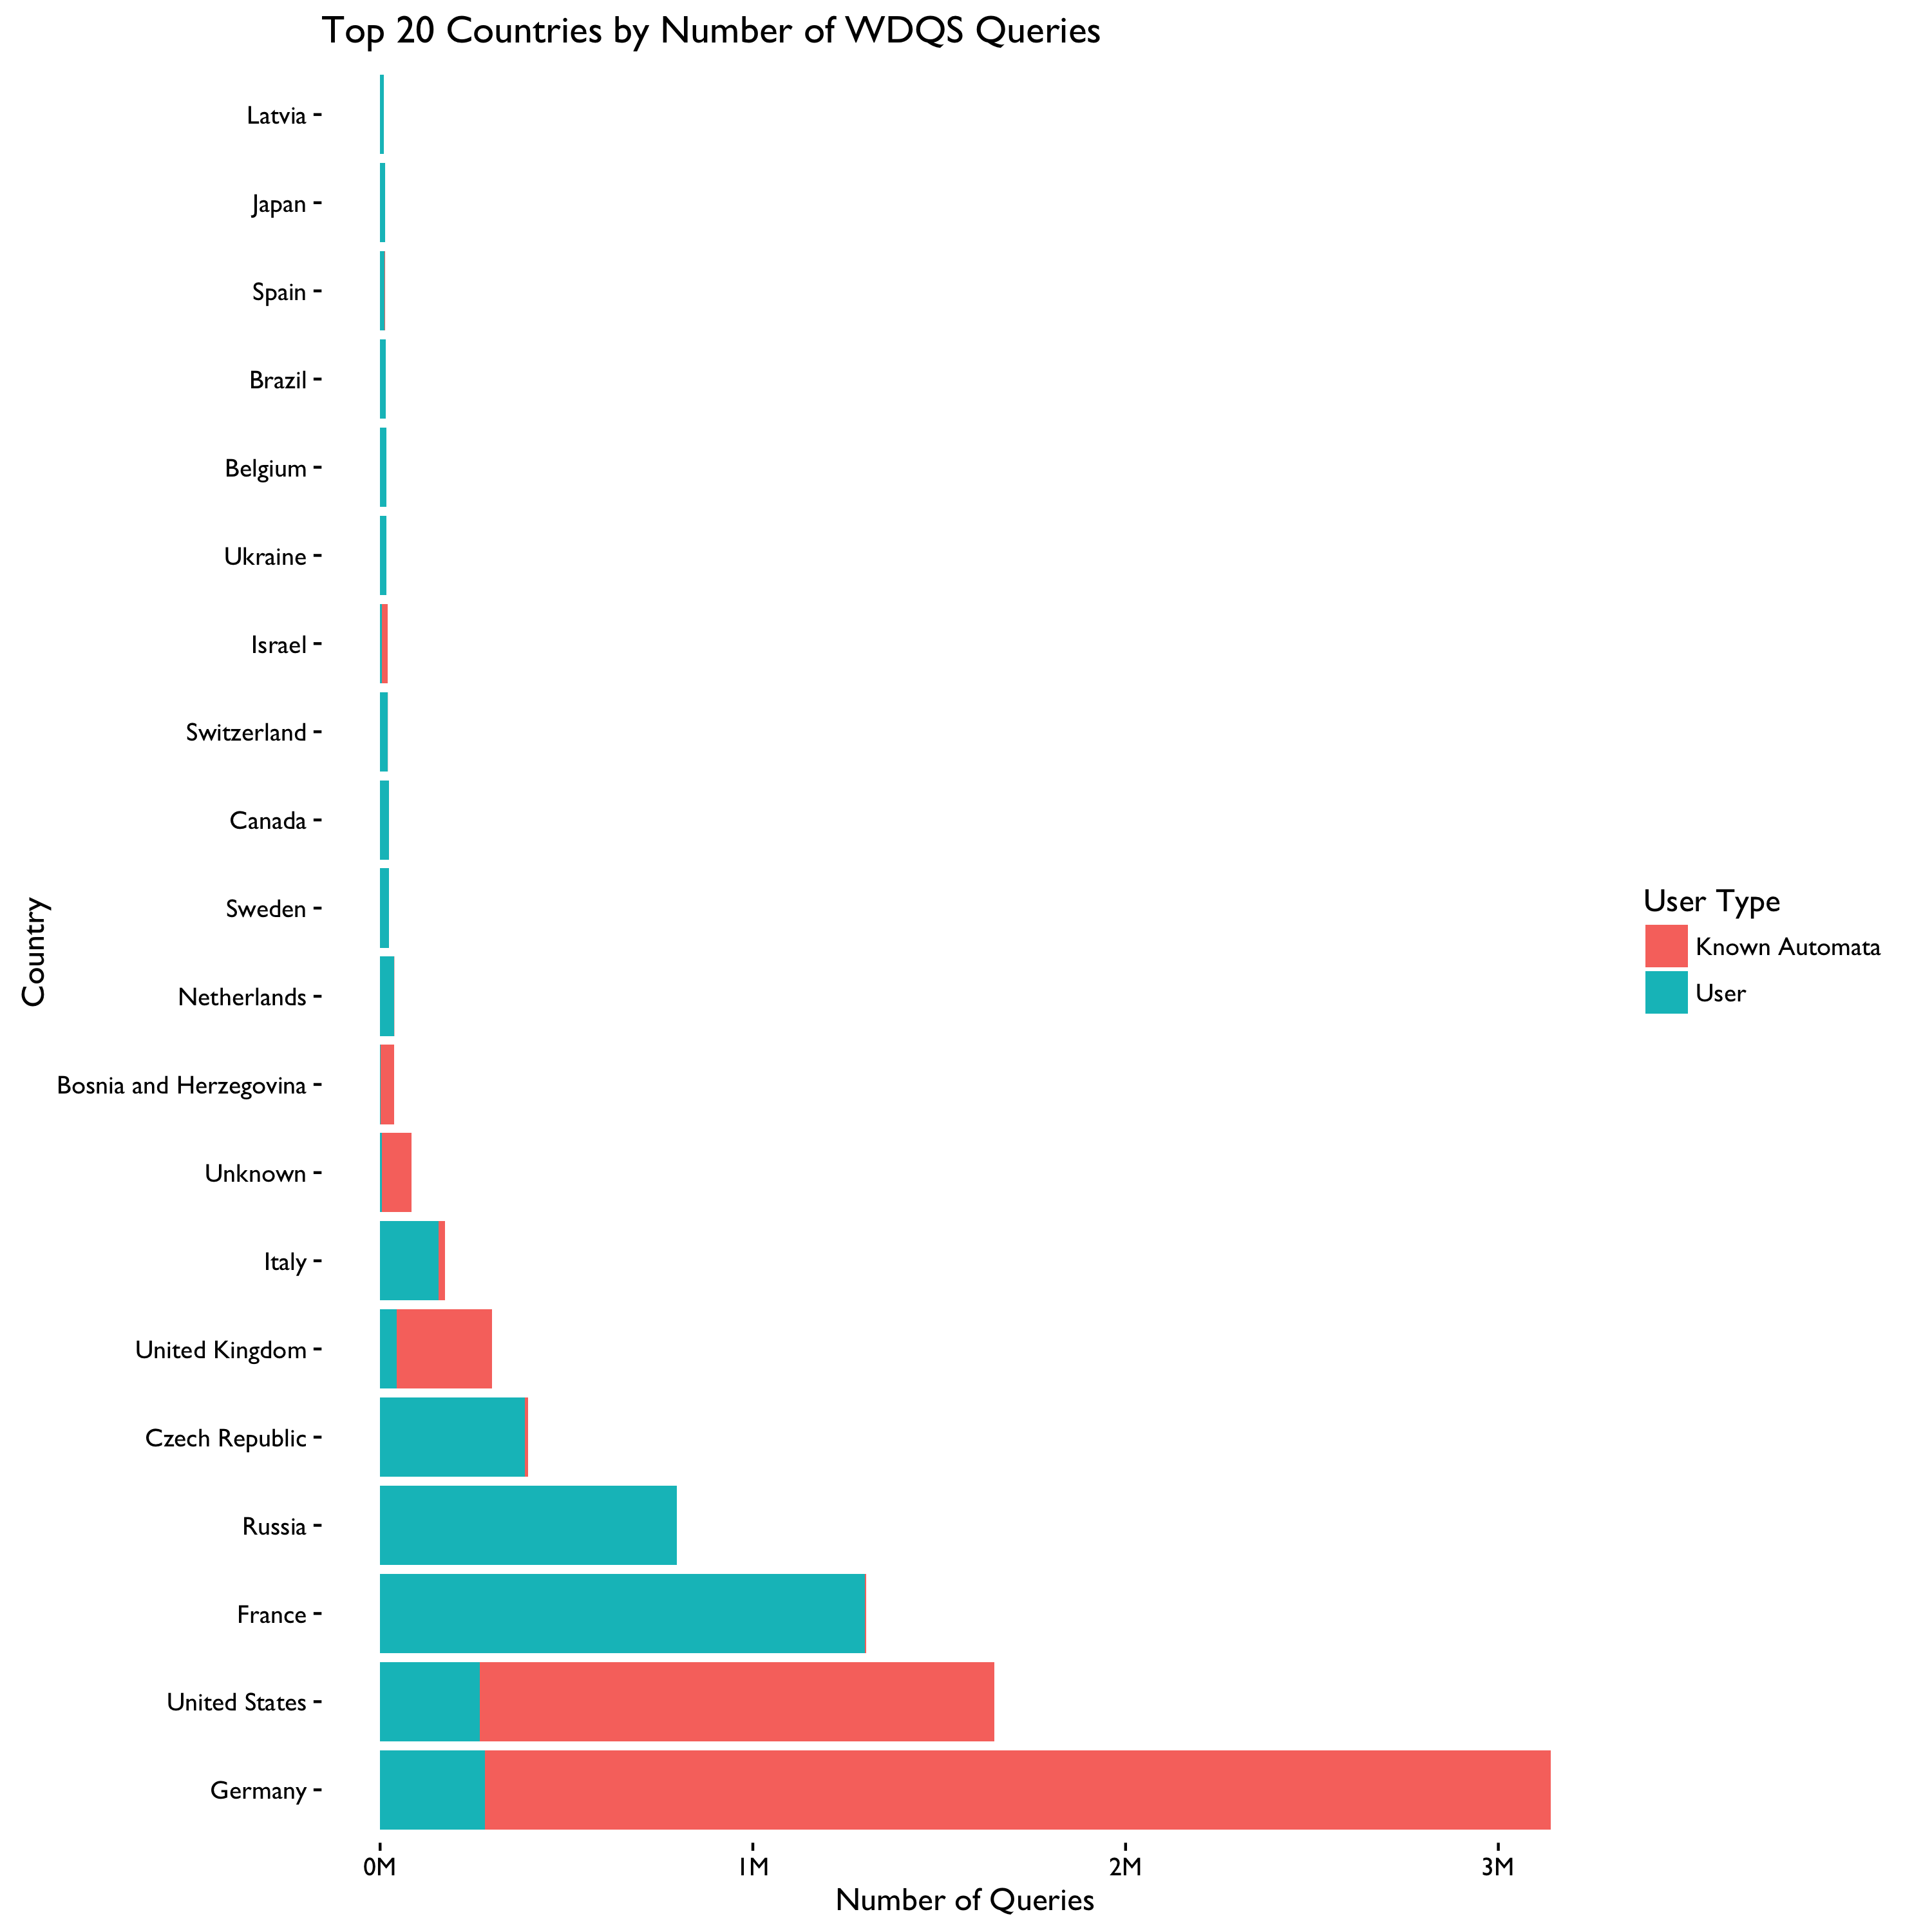
\includegraphics{figures/n_query_by_country.png}
\caption{Germany, United States and France take the first 3 places on
the rank. While most of them are automata queries in Germany and US,
France has the most user queries.}
\end{figure}

\begin{figure}[H]
\centering
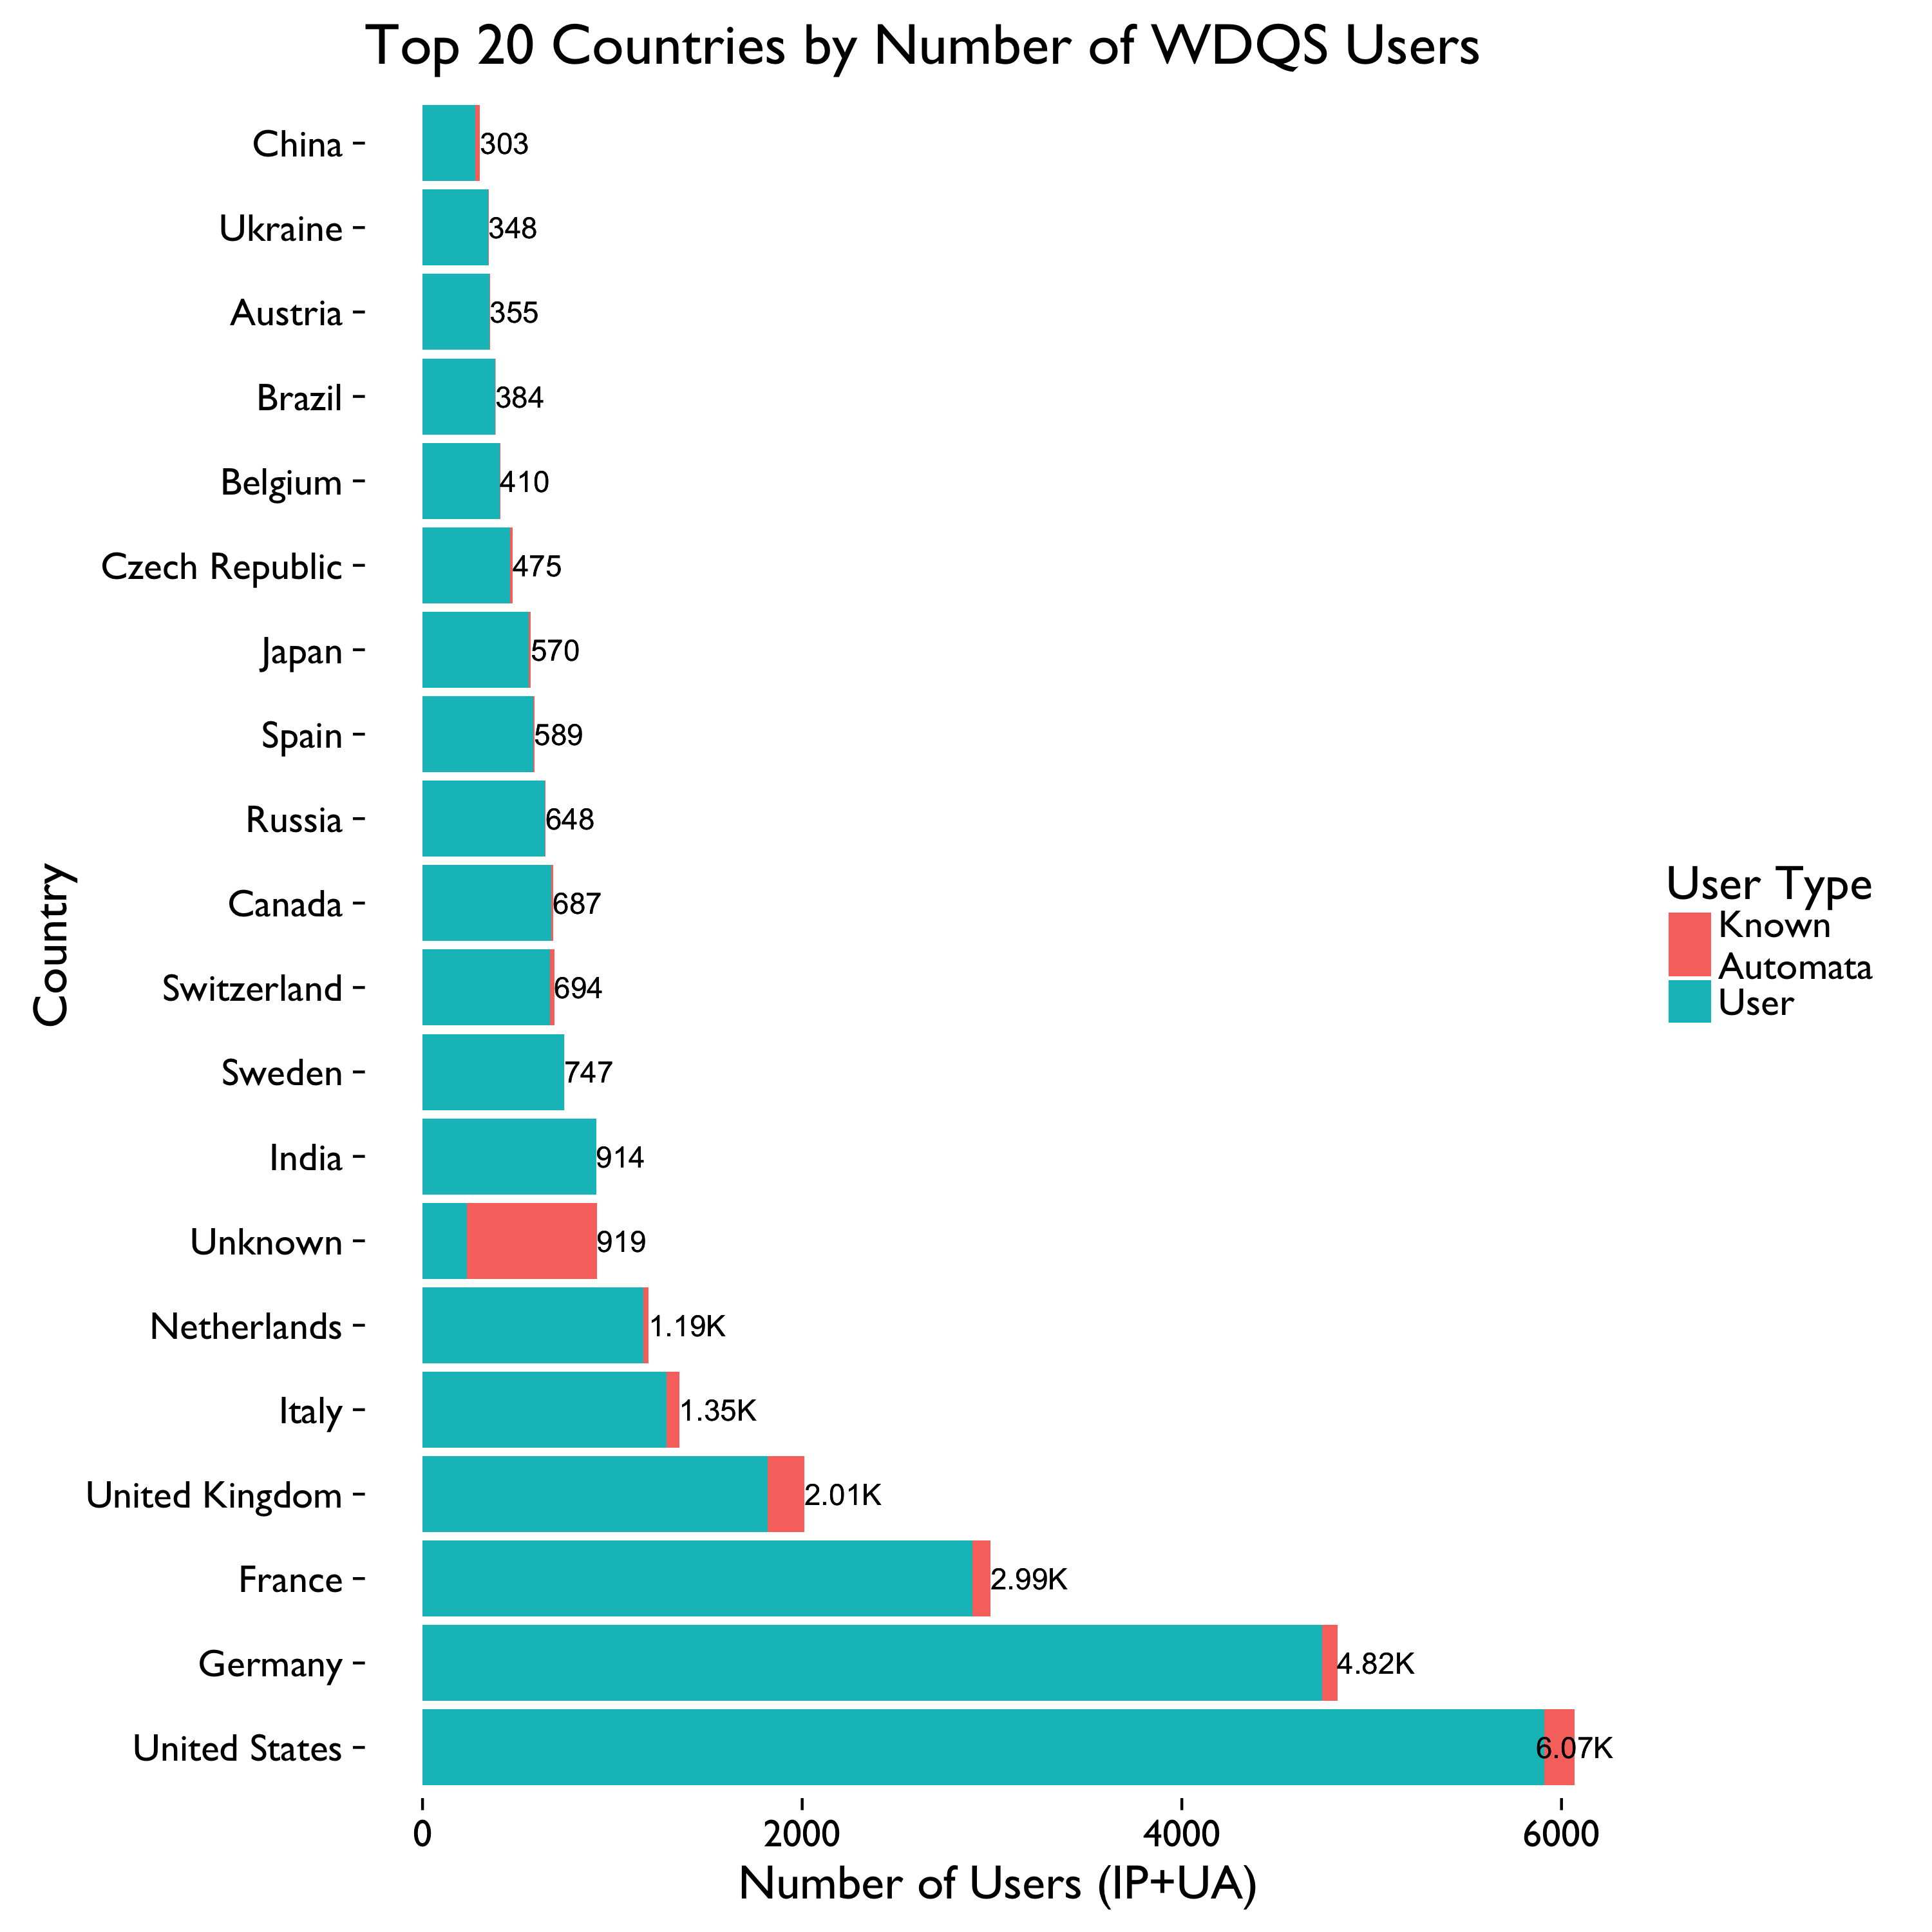
\includegraphics{figures/n_user_by_country.png}
\caption{United States, Germany and France have the largest number of
WDQS users.}
\end{figure}

\begin{figure}[H]
\centering
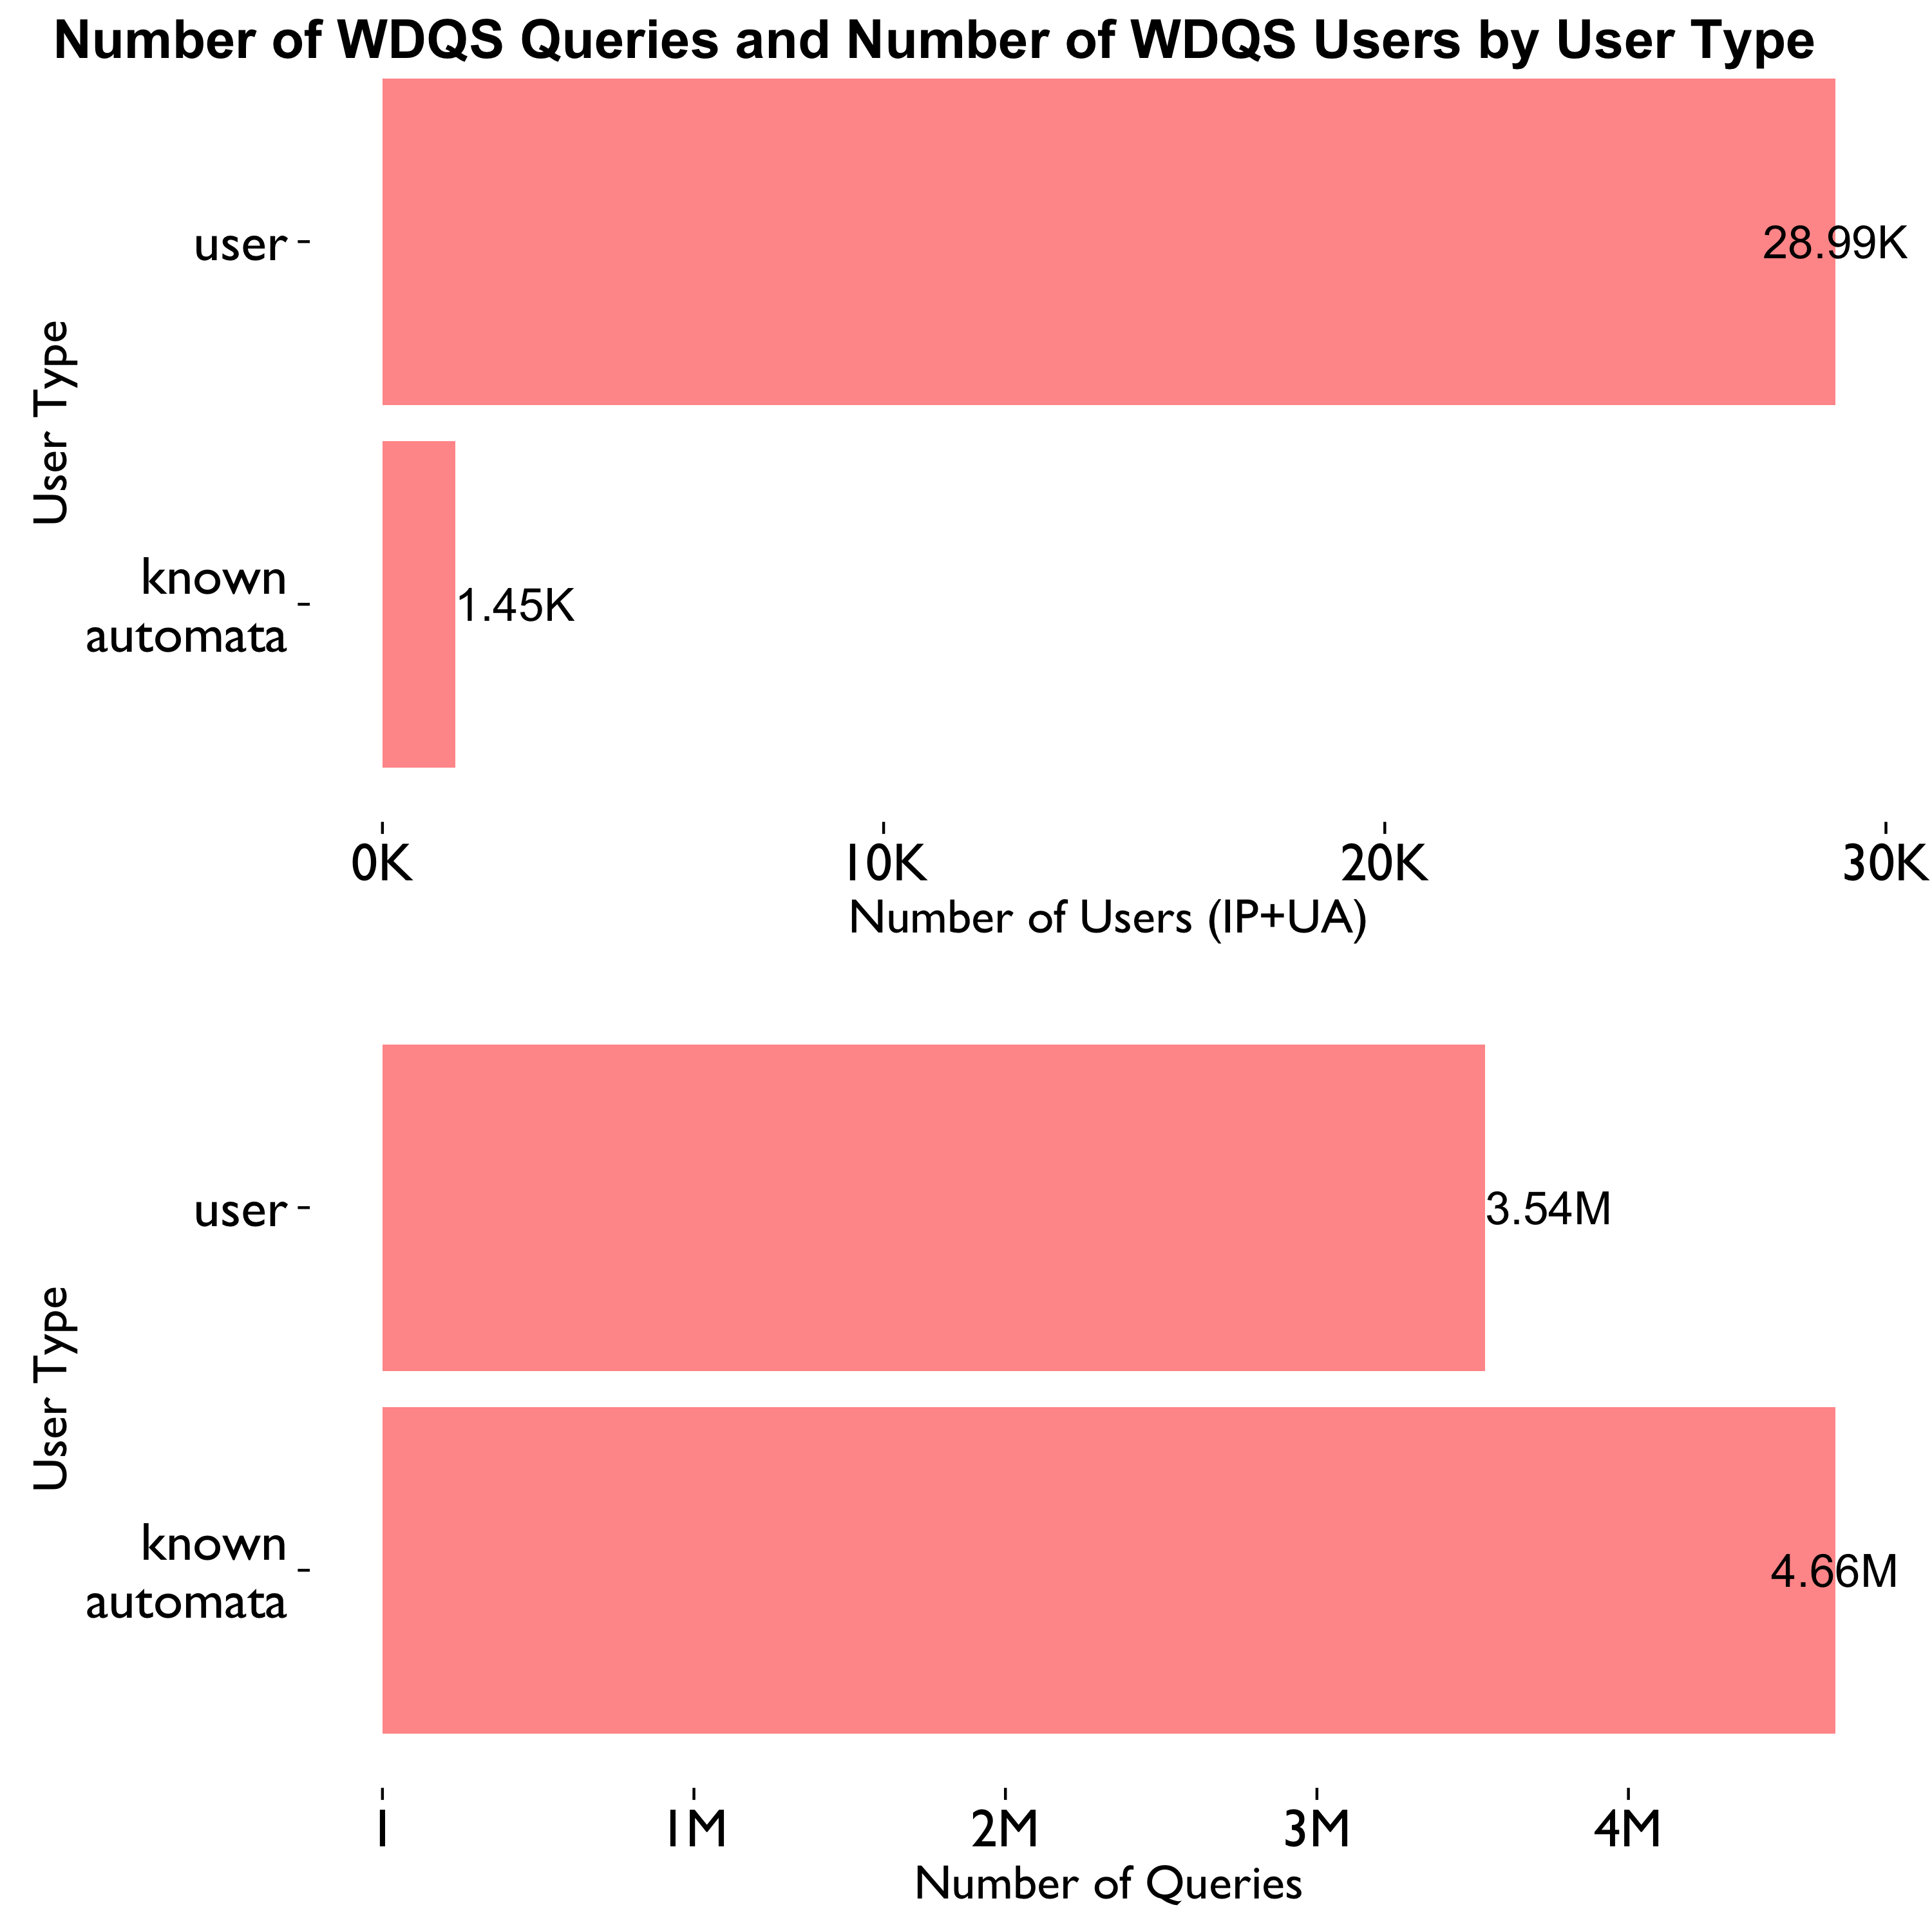
\includegraphics[width=11cm,height=11cm,keepaspectratio]{figures/by_agent_type.png}
\caption{Number of WDQS Queries and Number of WDQS Users by User Type.}
\end{figure}

\begin{figure}[H]
\centering
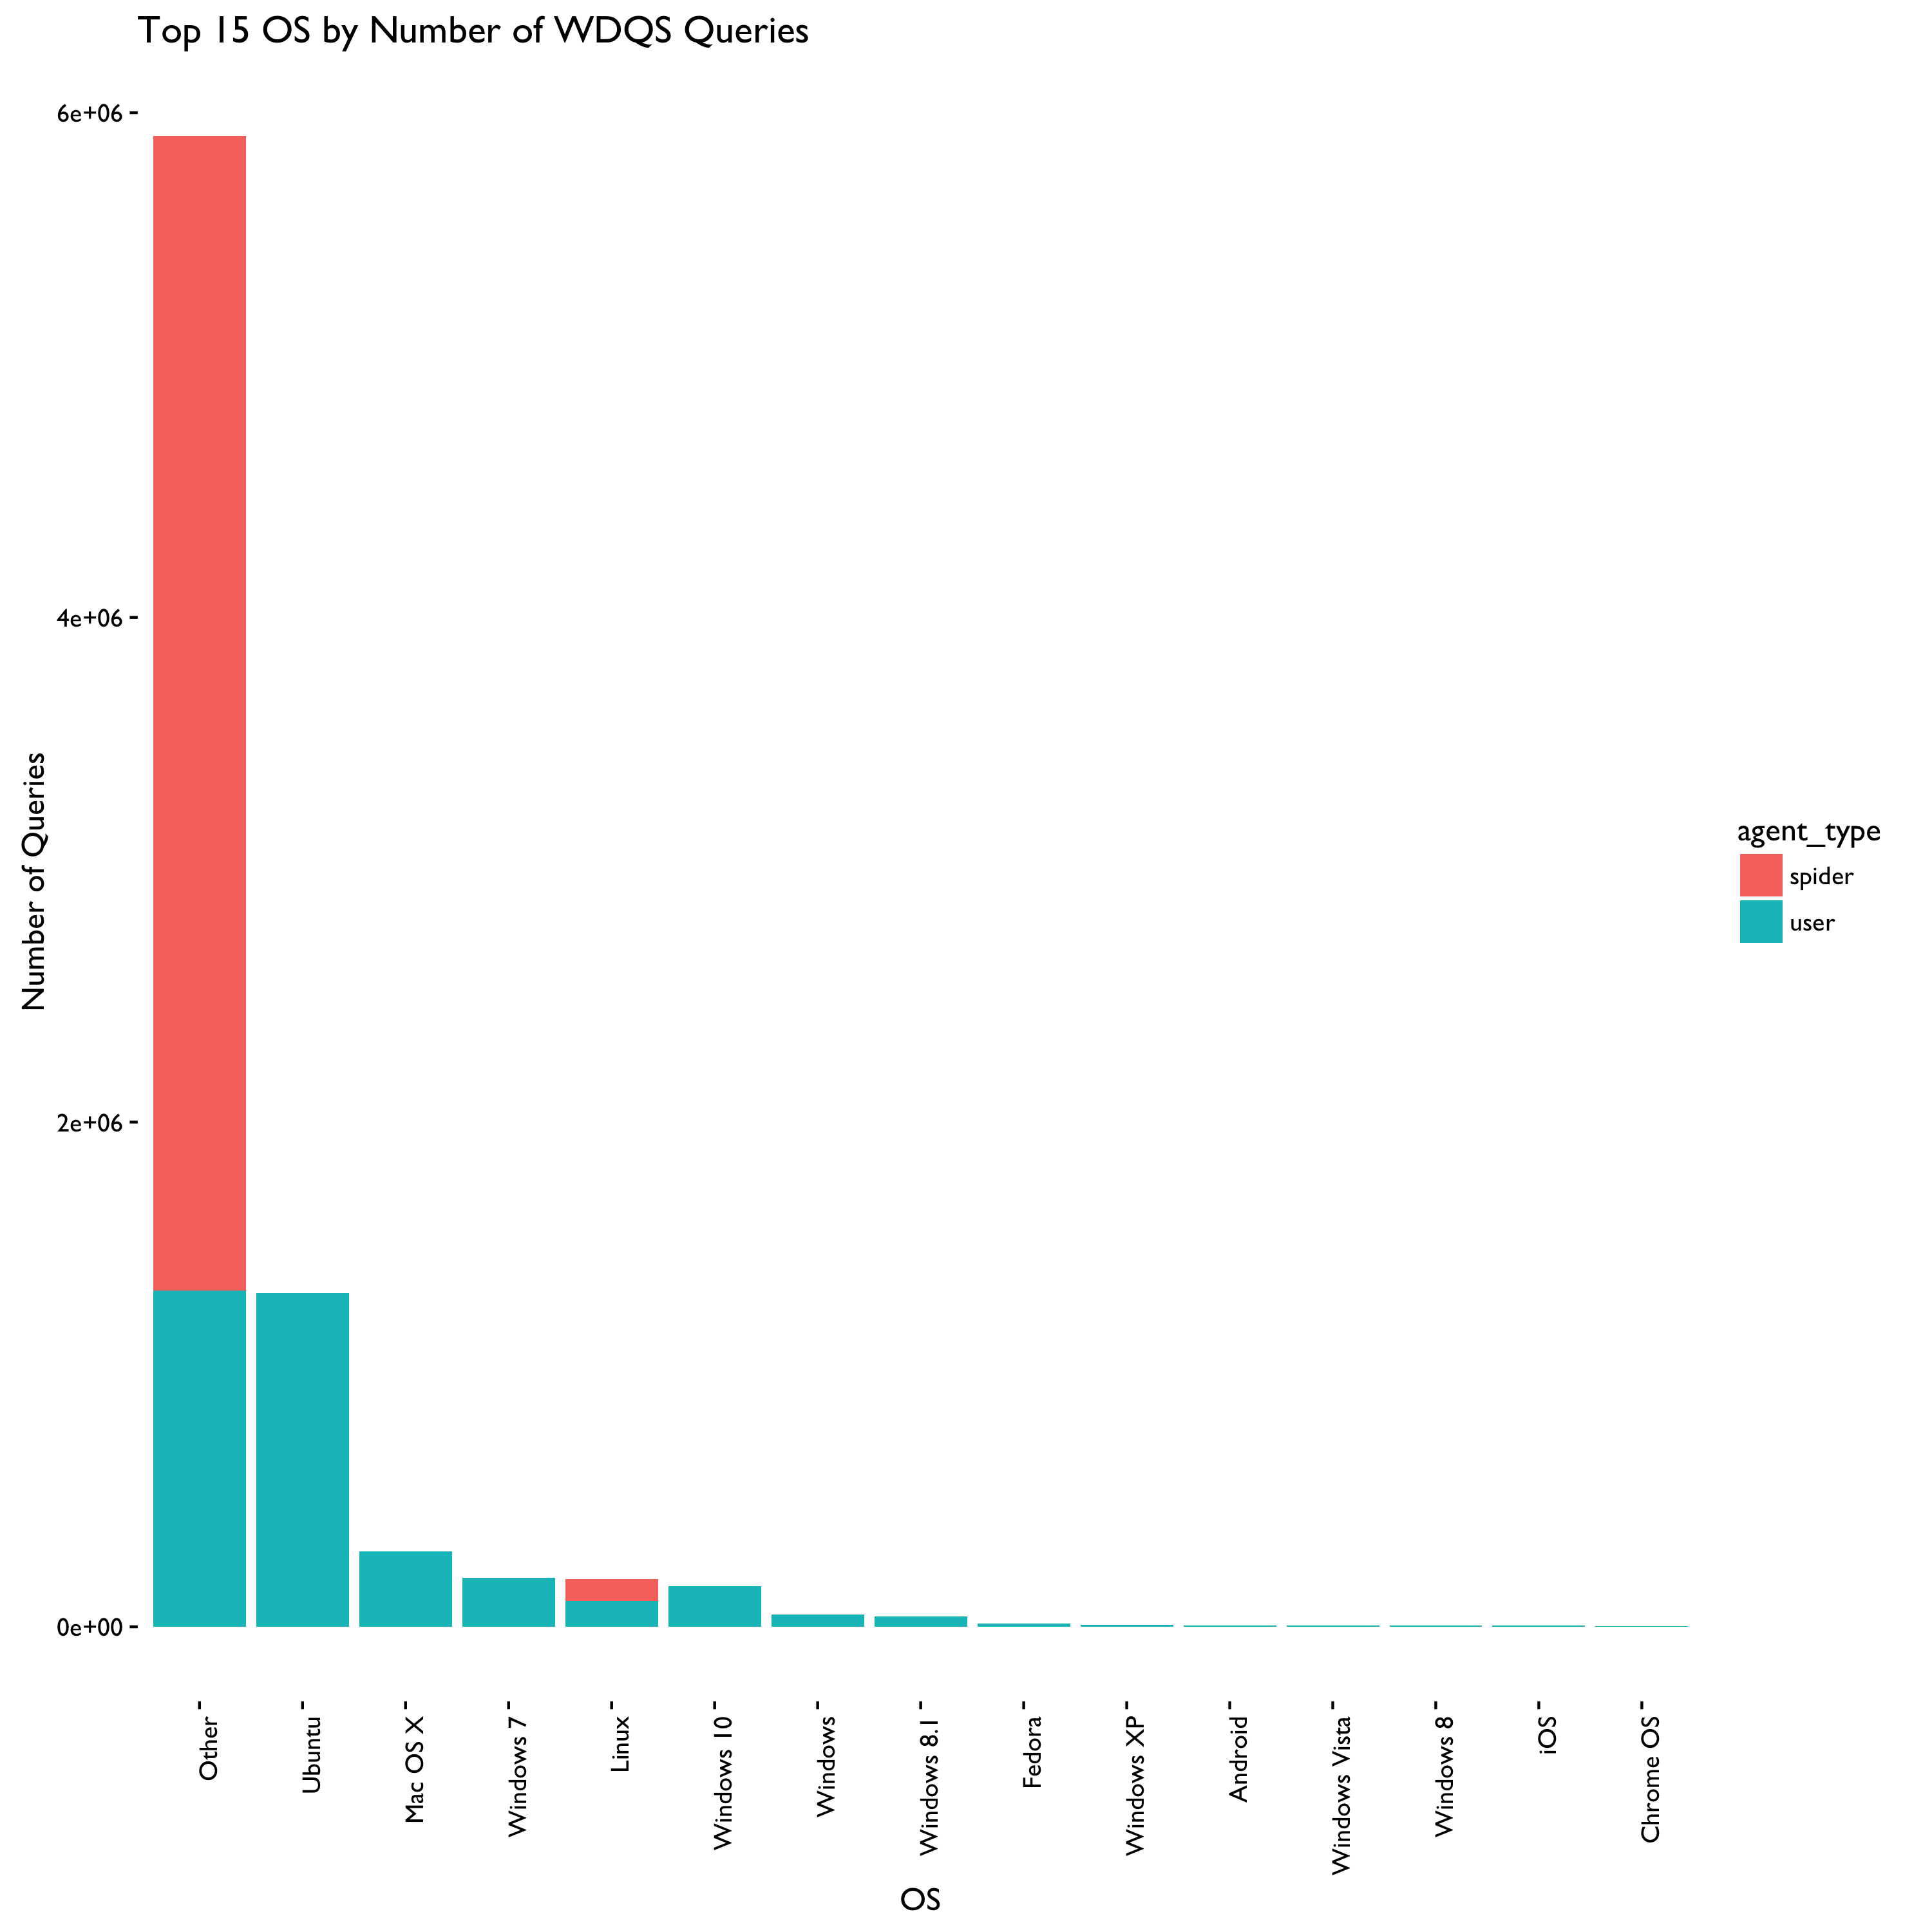
\includegraphics[width=11cm,height=11cm,keepaspectratio]{figures/n_query_by_os.png}
\caption{Top 15 Operating Systems by Number of WDQS Queries, Excluding
Known Automata.}
\end{figure}

\begin{figure}[H]
\centering
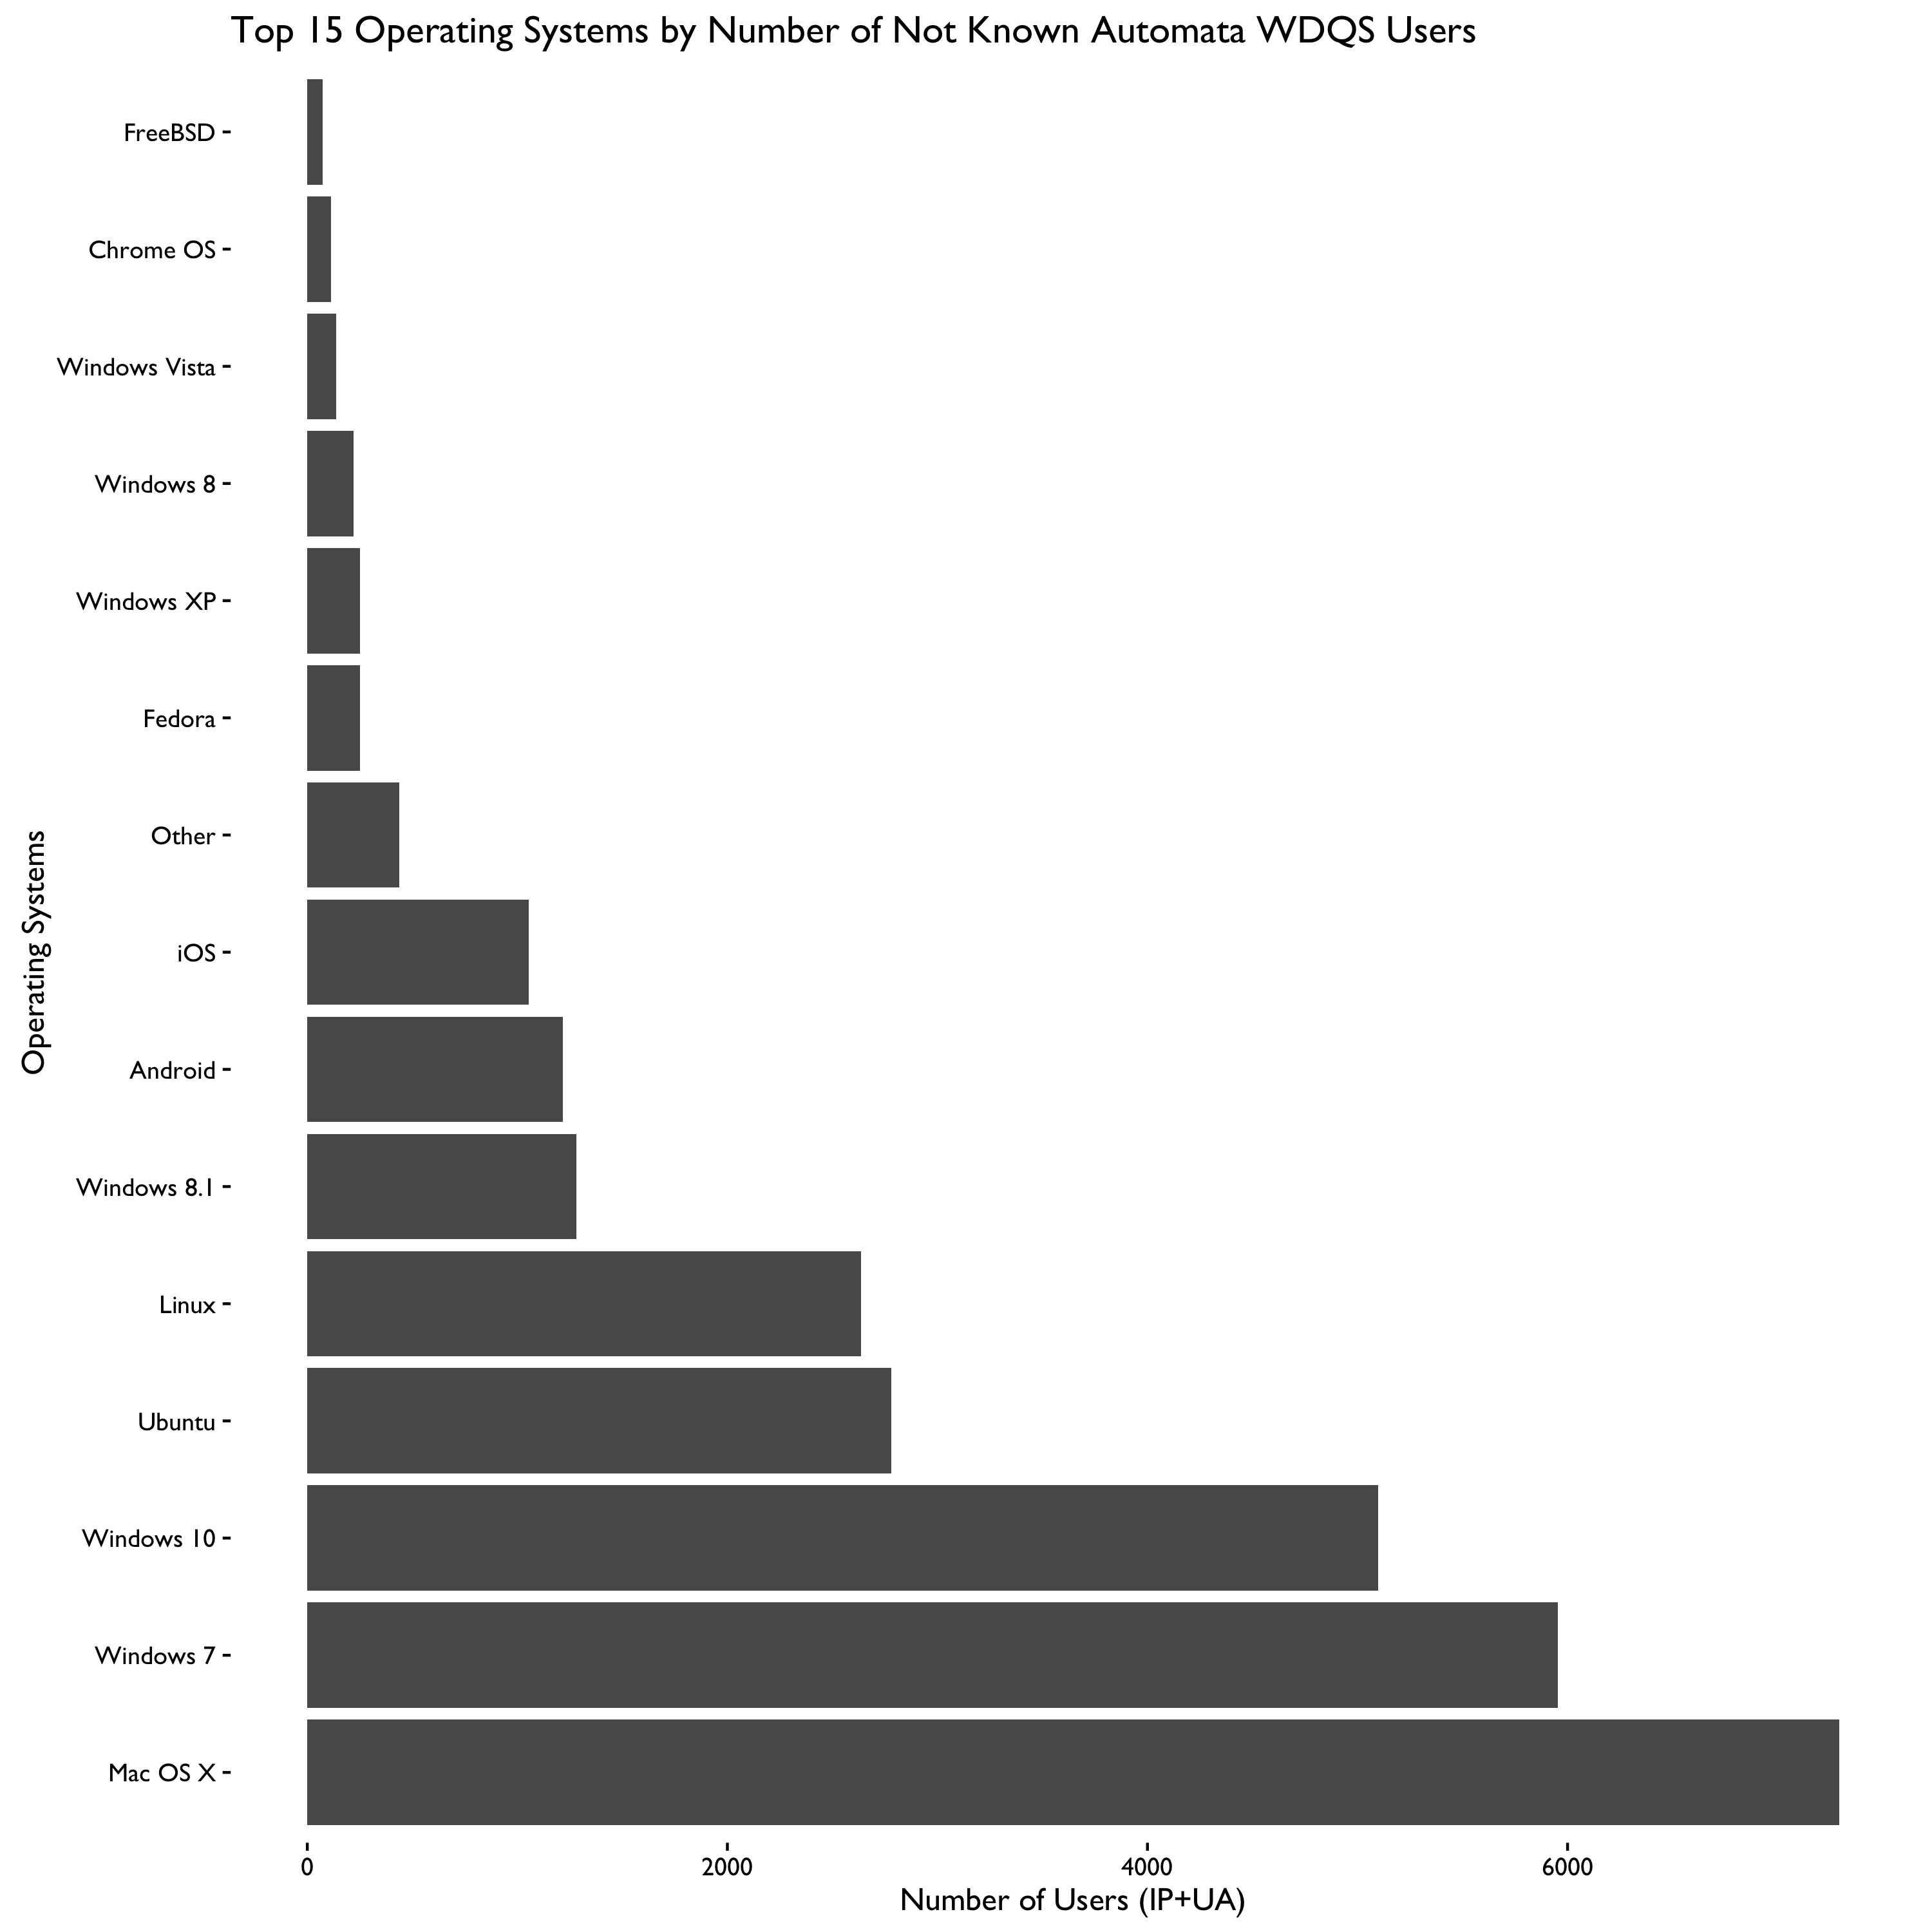
\includegraphics[width=11cm,height=11cm,keepaspectratio]{figures/n_user_by_os.png}
\caption{Top 15 Operating Systems by Number of WDQS Users, Excluding
Known Automata. It looks like Ubuntu users have more queries-per-user
than other operating systems on average.}
\end{figure}

\begin{figure}[H]
\centering
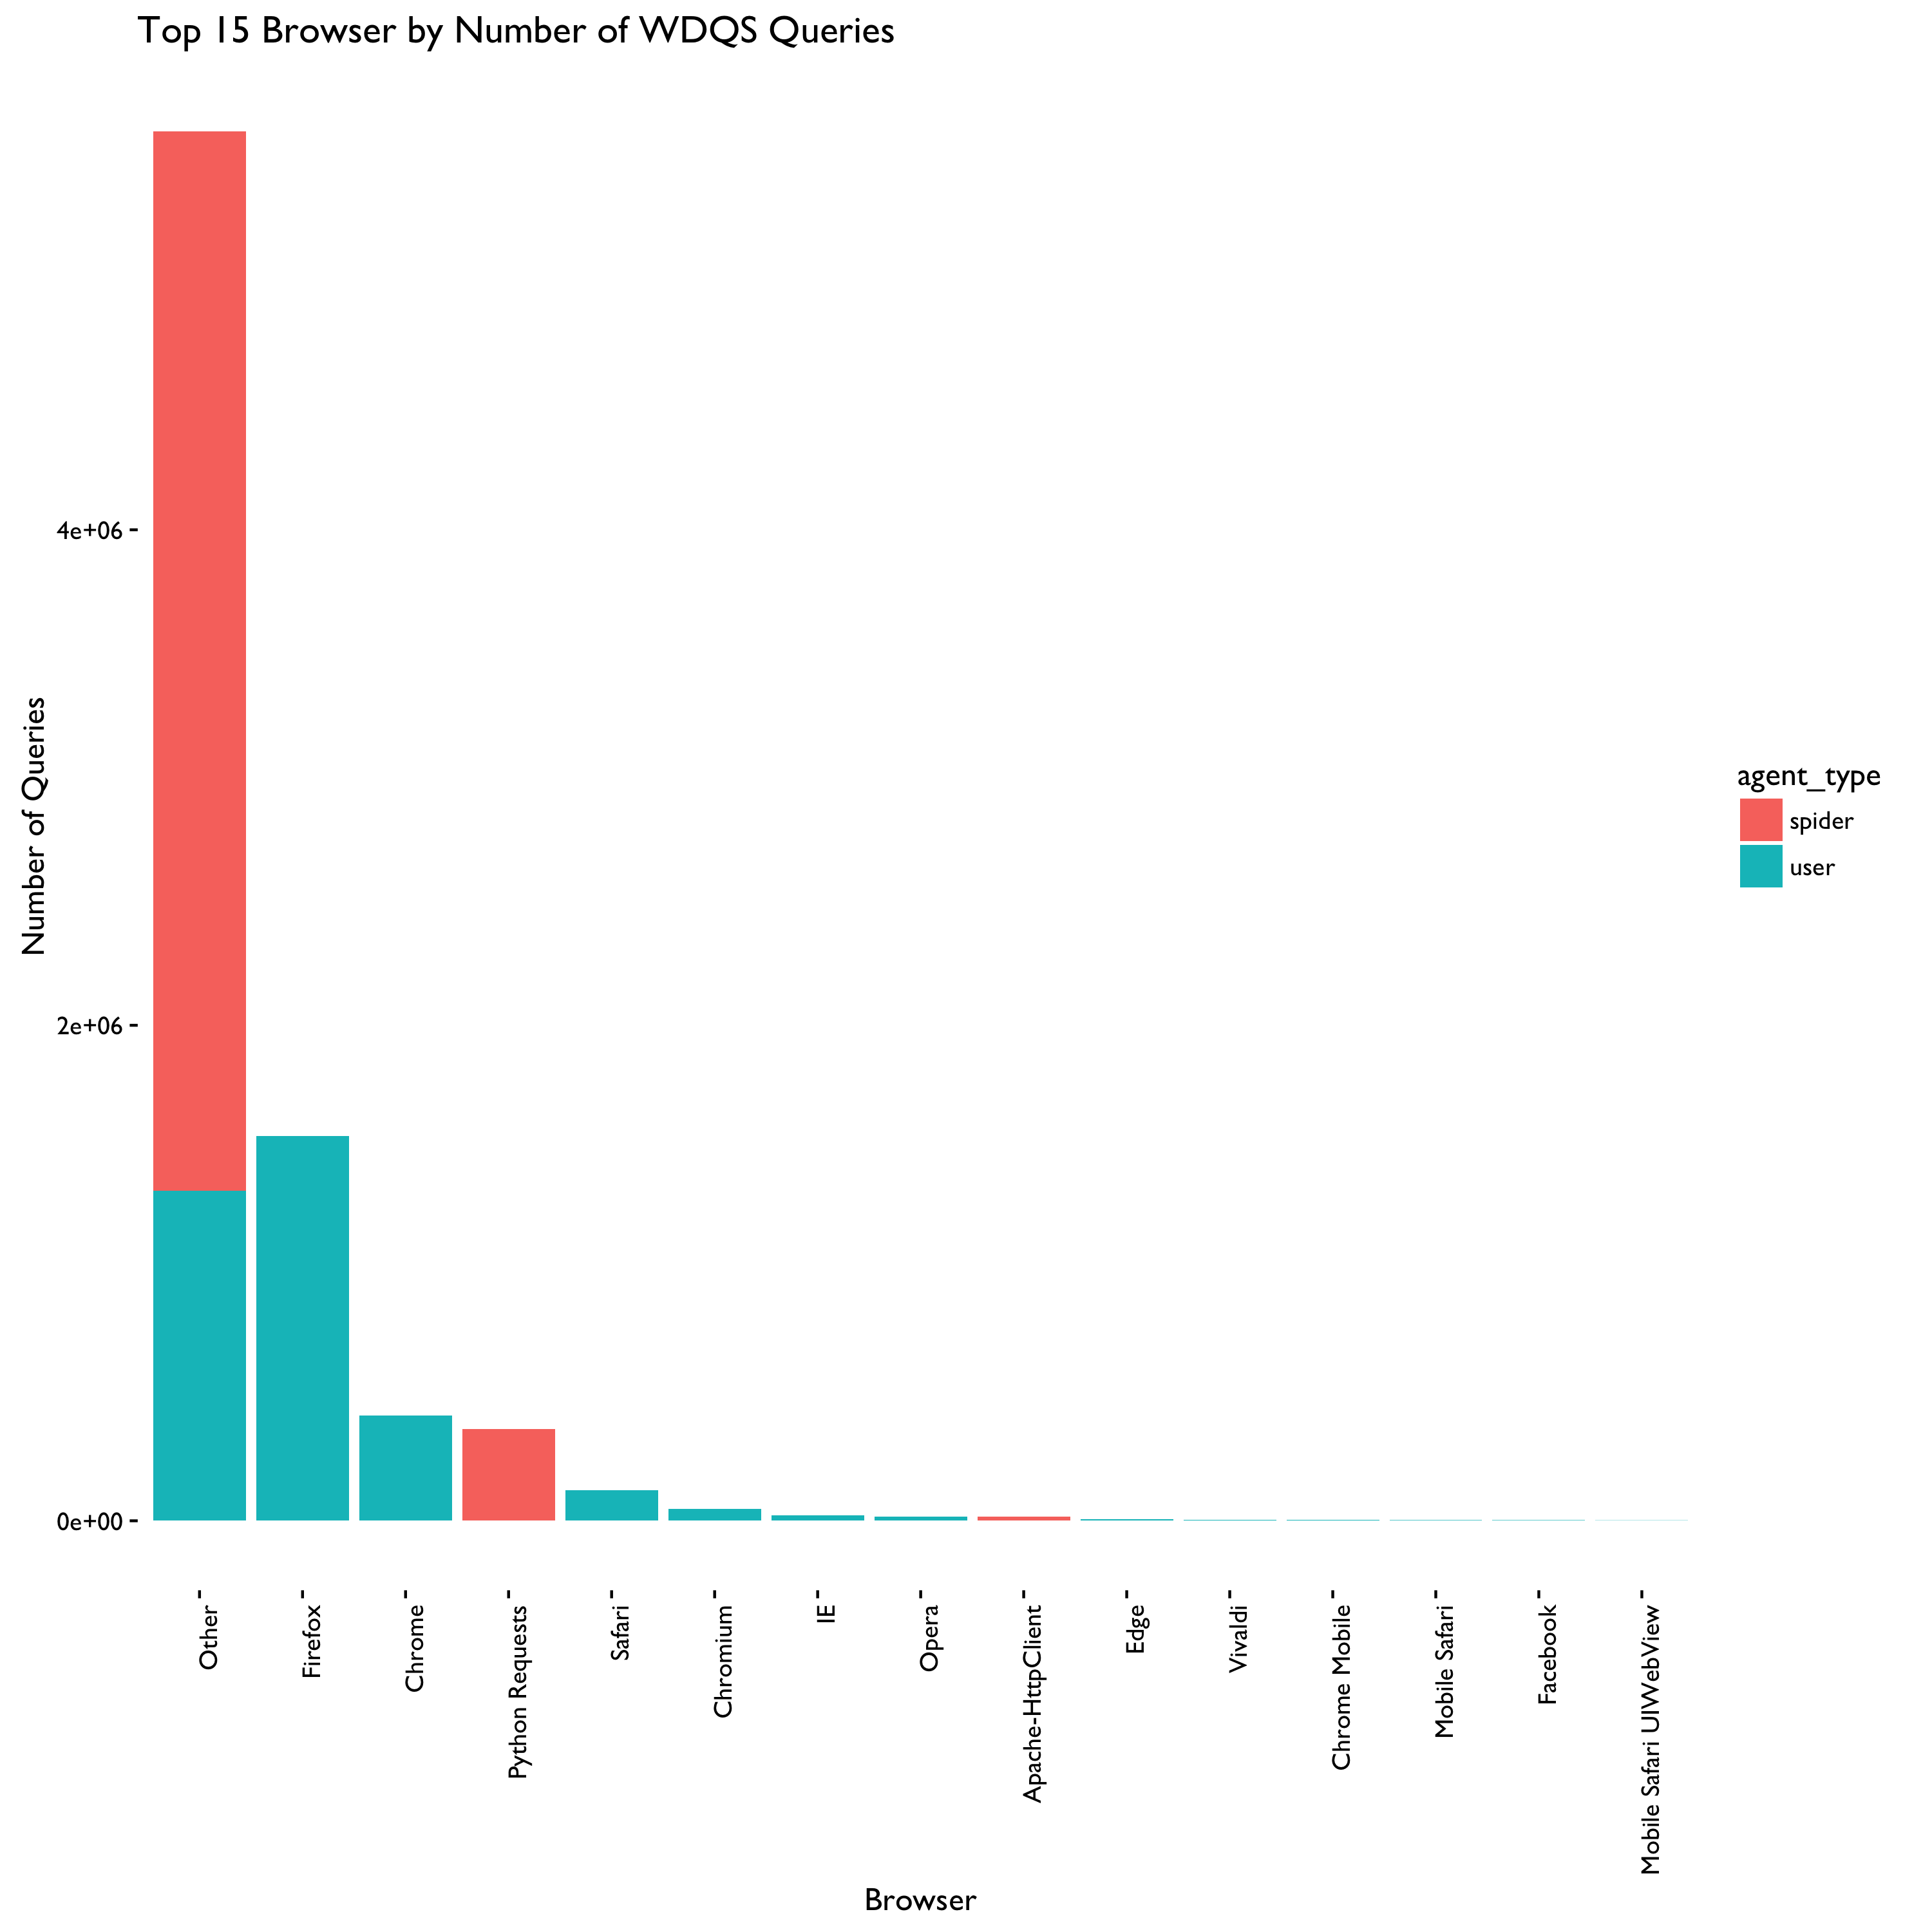
\includegraphics[width=11cm,height=11cm,keepaspectratio]{figures/n_query_by_browser.png}
\caption{Top 15 Browser by Number of WDQS Queries, Excluding Known
Automata.}
\end{figure}

\begin{figure}[H]
\centering
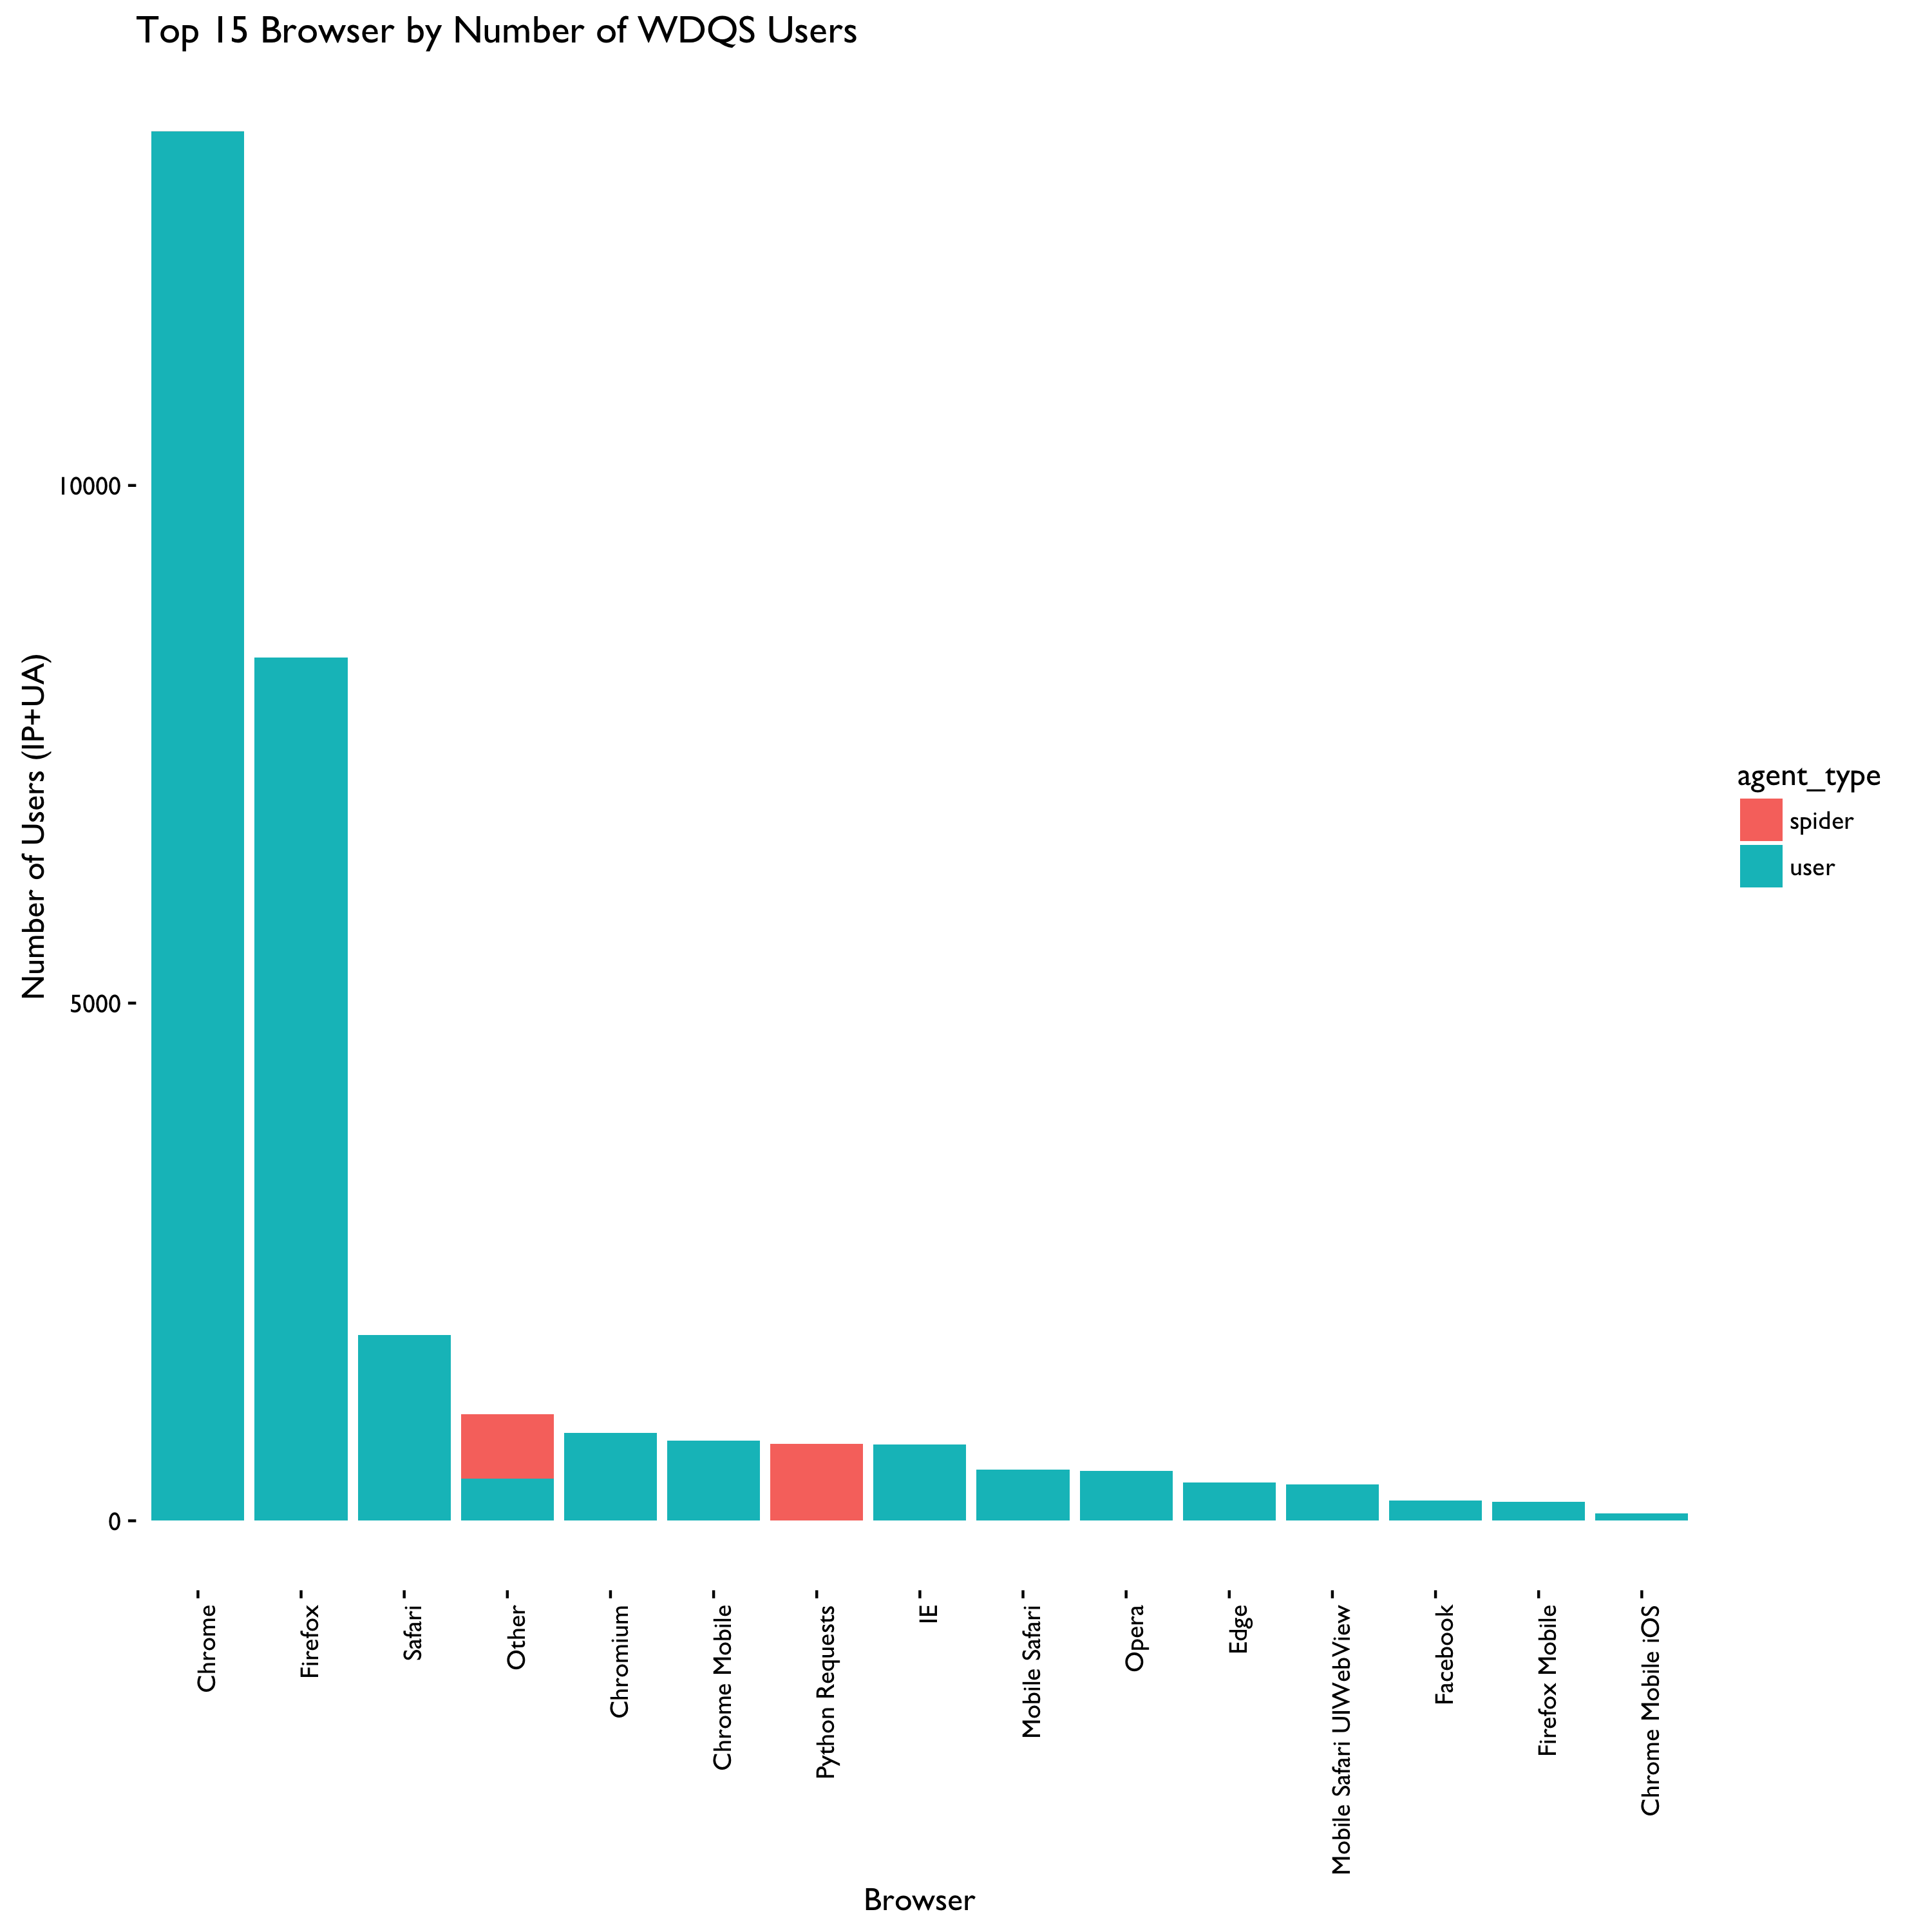
\includegraphics[width=11cm,height=11cm,keepaspectratio]{figures/n_user_by_browser.png}
\caption{Top 15 Browser by Number of WDQS Users, Excluding Known
Automata.}
\end{figure}

\begin{figure}[H]
\centering
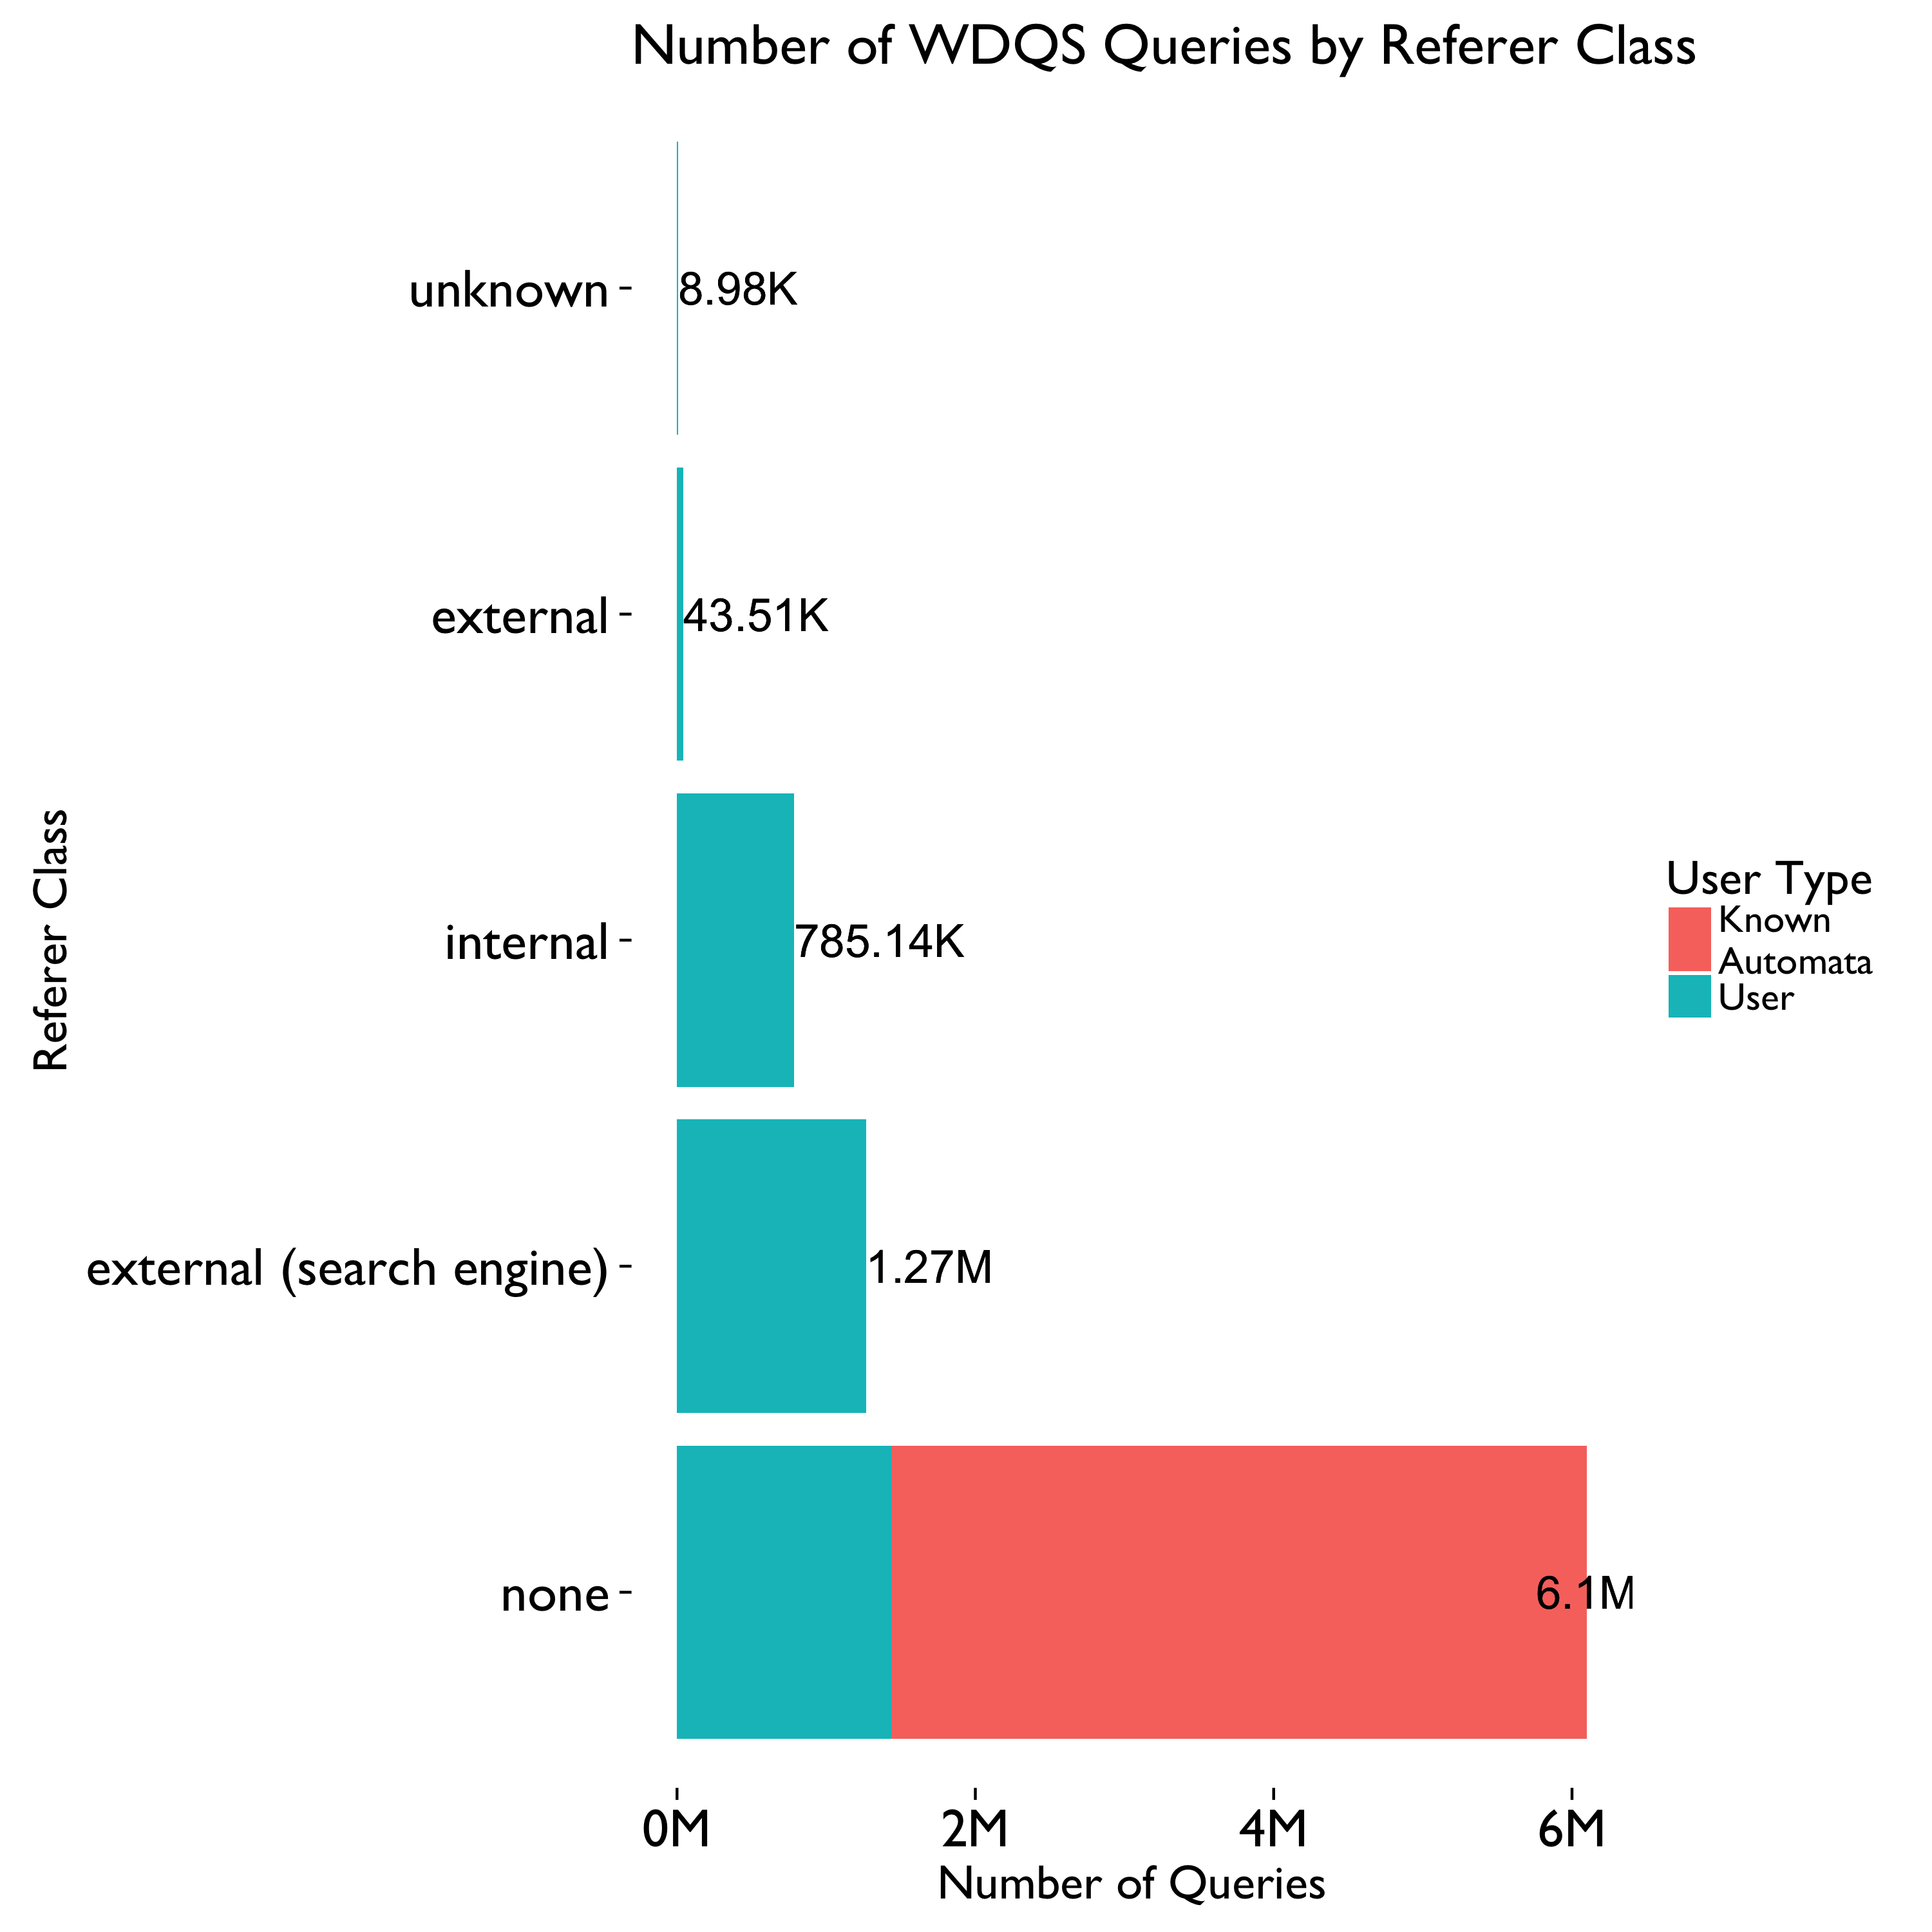
\includegraphics[width=10cm,height=10cm,keepaspectratio]{figures/n_query_by_referer_class.png}
\caption{Most queries do not have a referer as they are from real
people, but there are a large amount of queries that are from automata.}
\end{figure}

\subsubsection{Longitudinal}\label{longitudinal}

\begin{figure}[H]
\centering
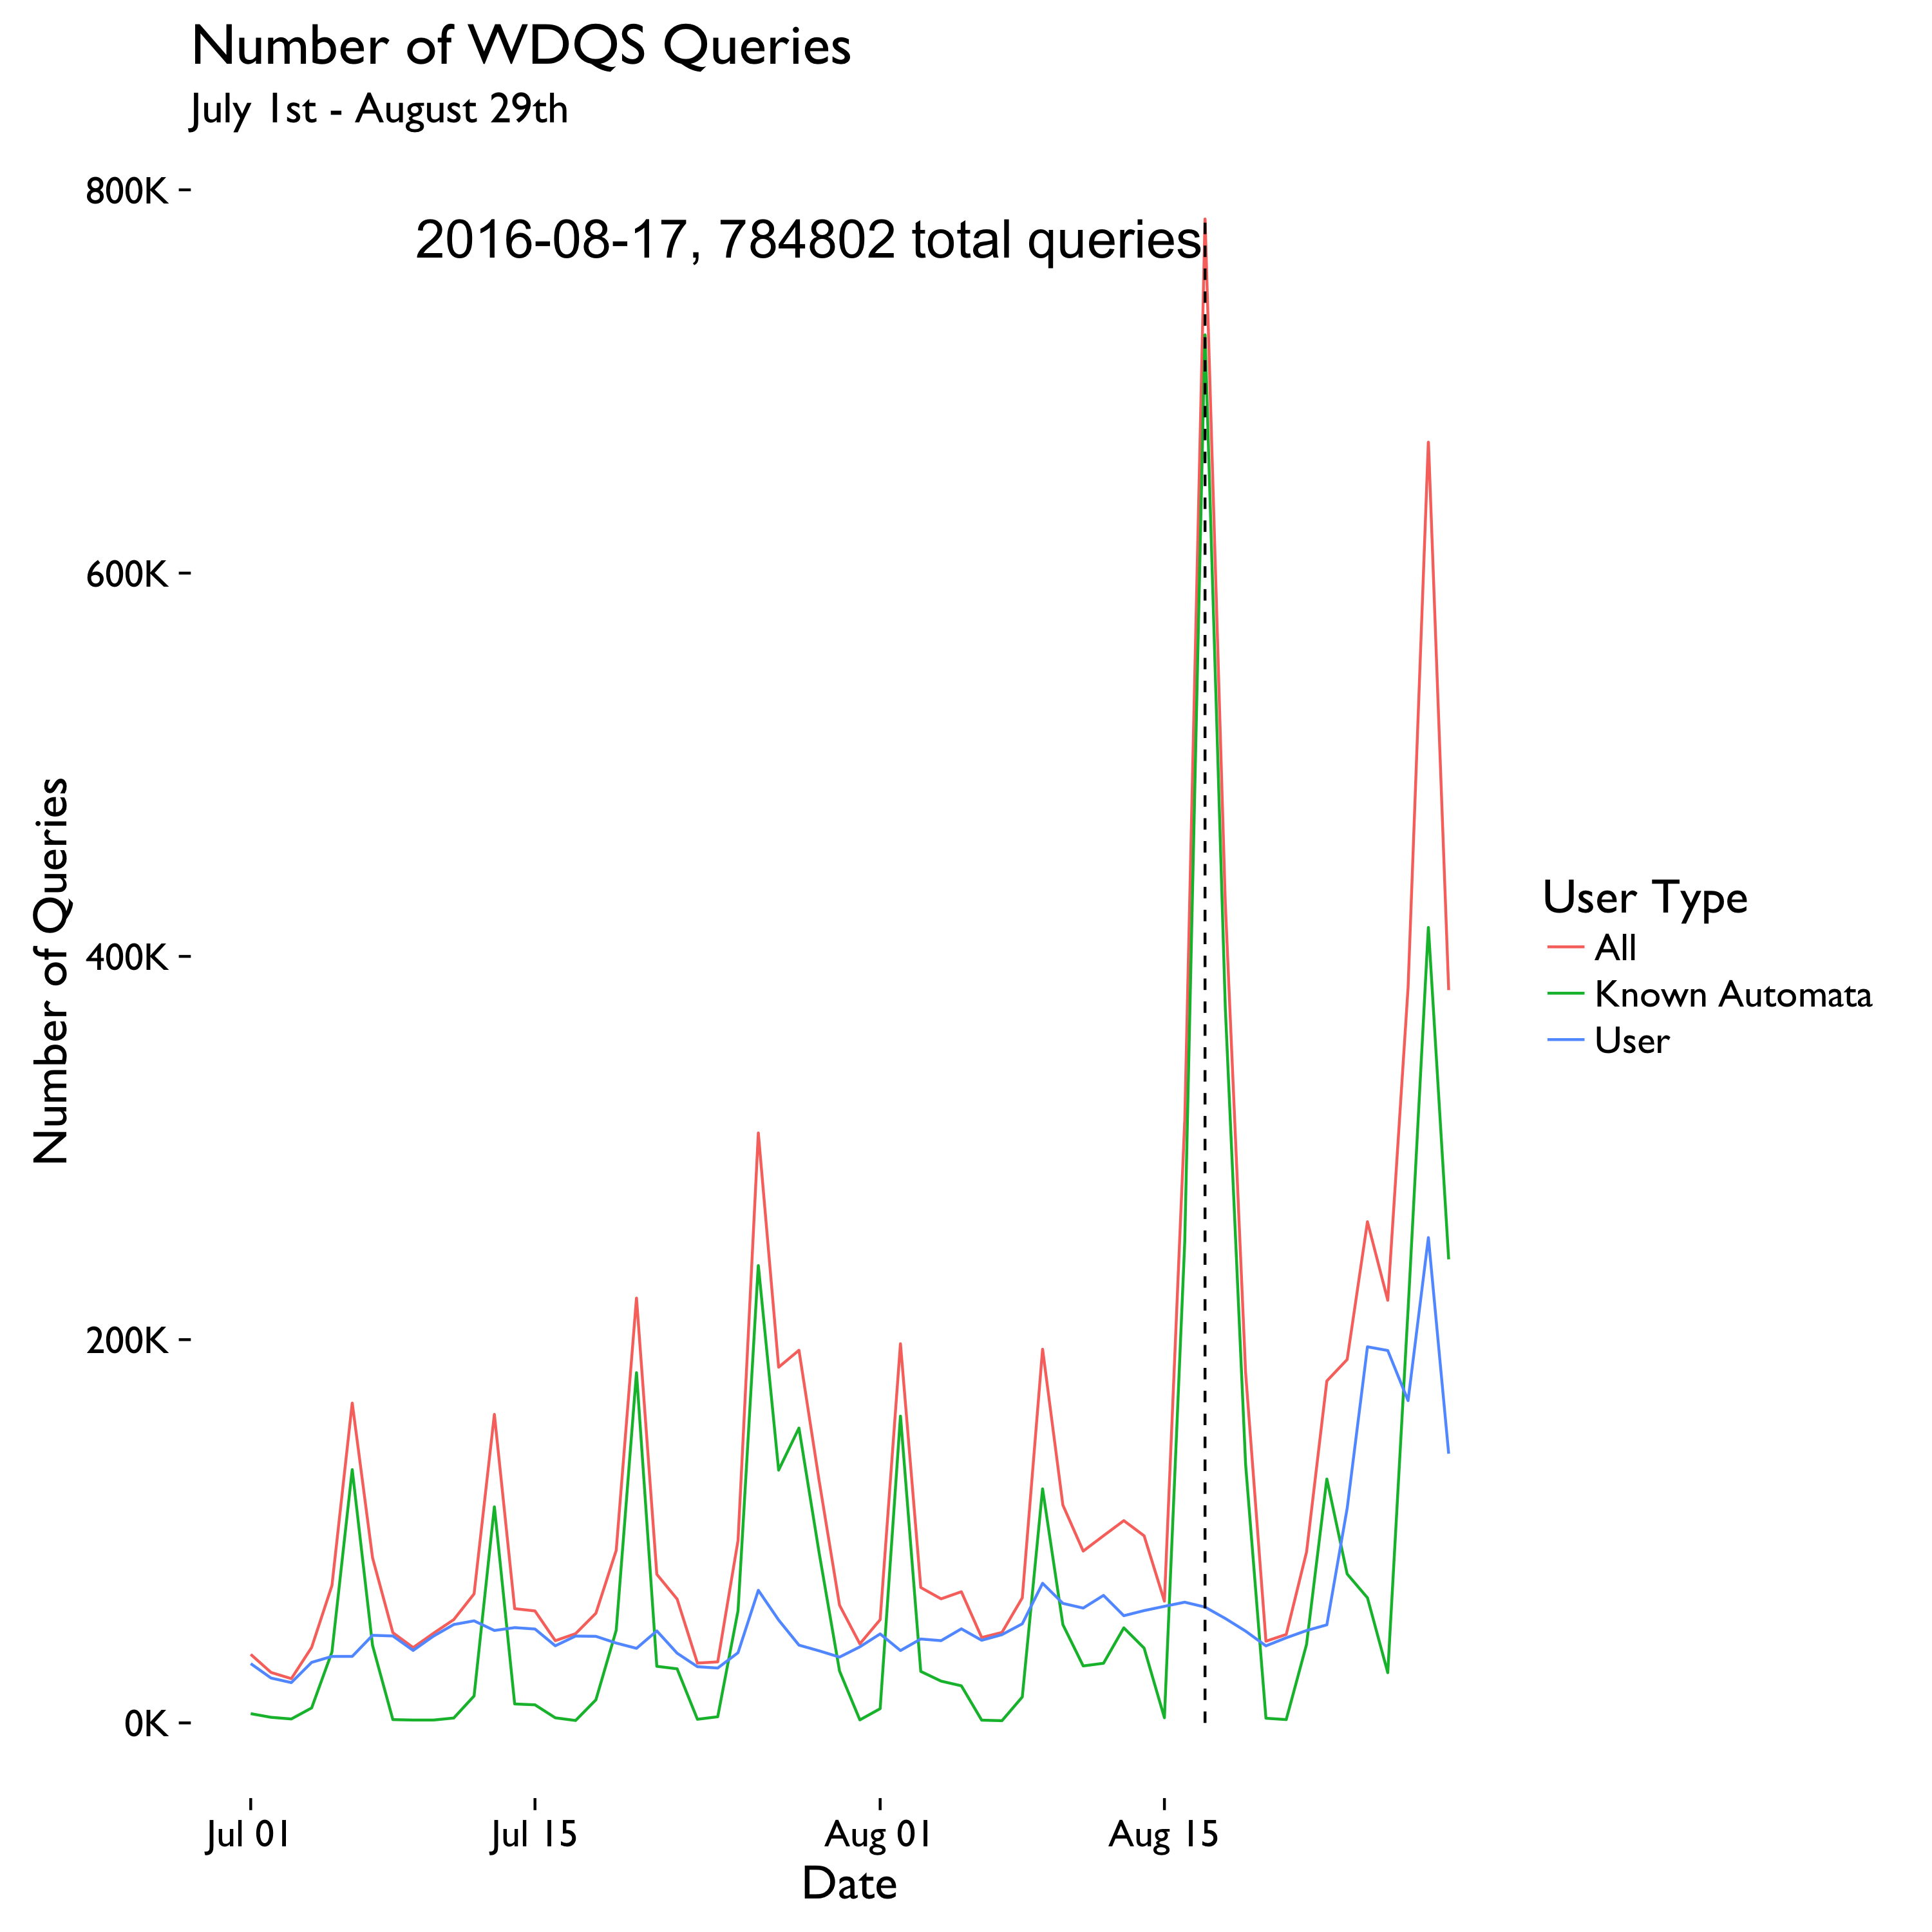
\includegraphics[width=9cm,height=9cm,keepaspectratio]{figures/all_query_ts.png}
\caption{There seems to be a weekly cycle in the number of automata
queries. After the spike (August 16-19), both types of queries saw an
increase.}
\end{figure}

\begin{figure}[H]
\centering
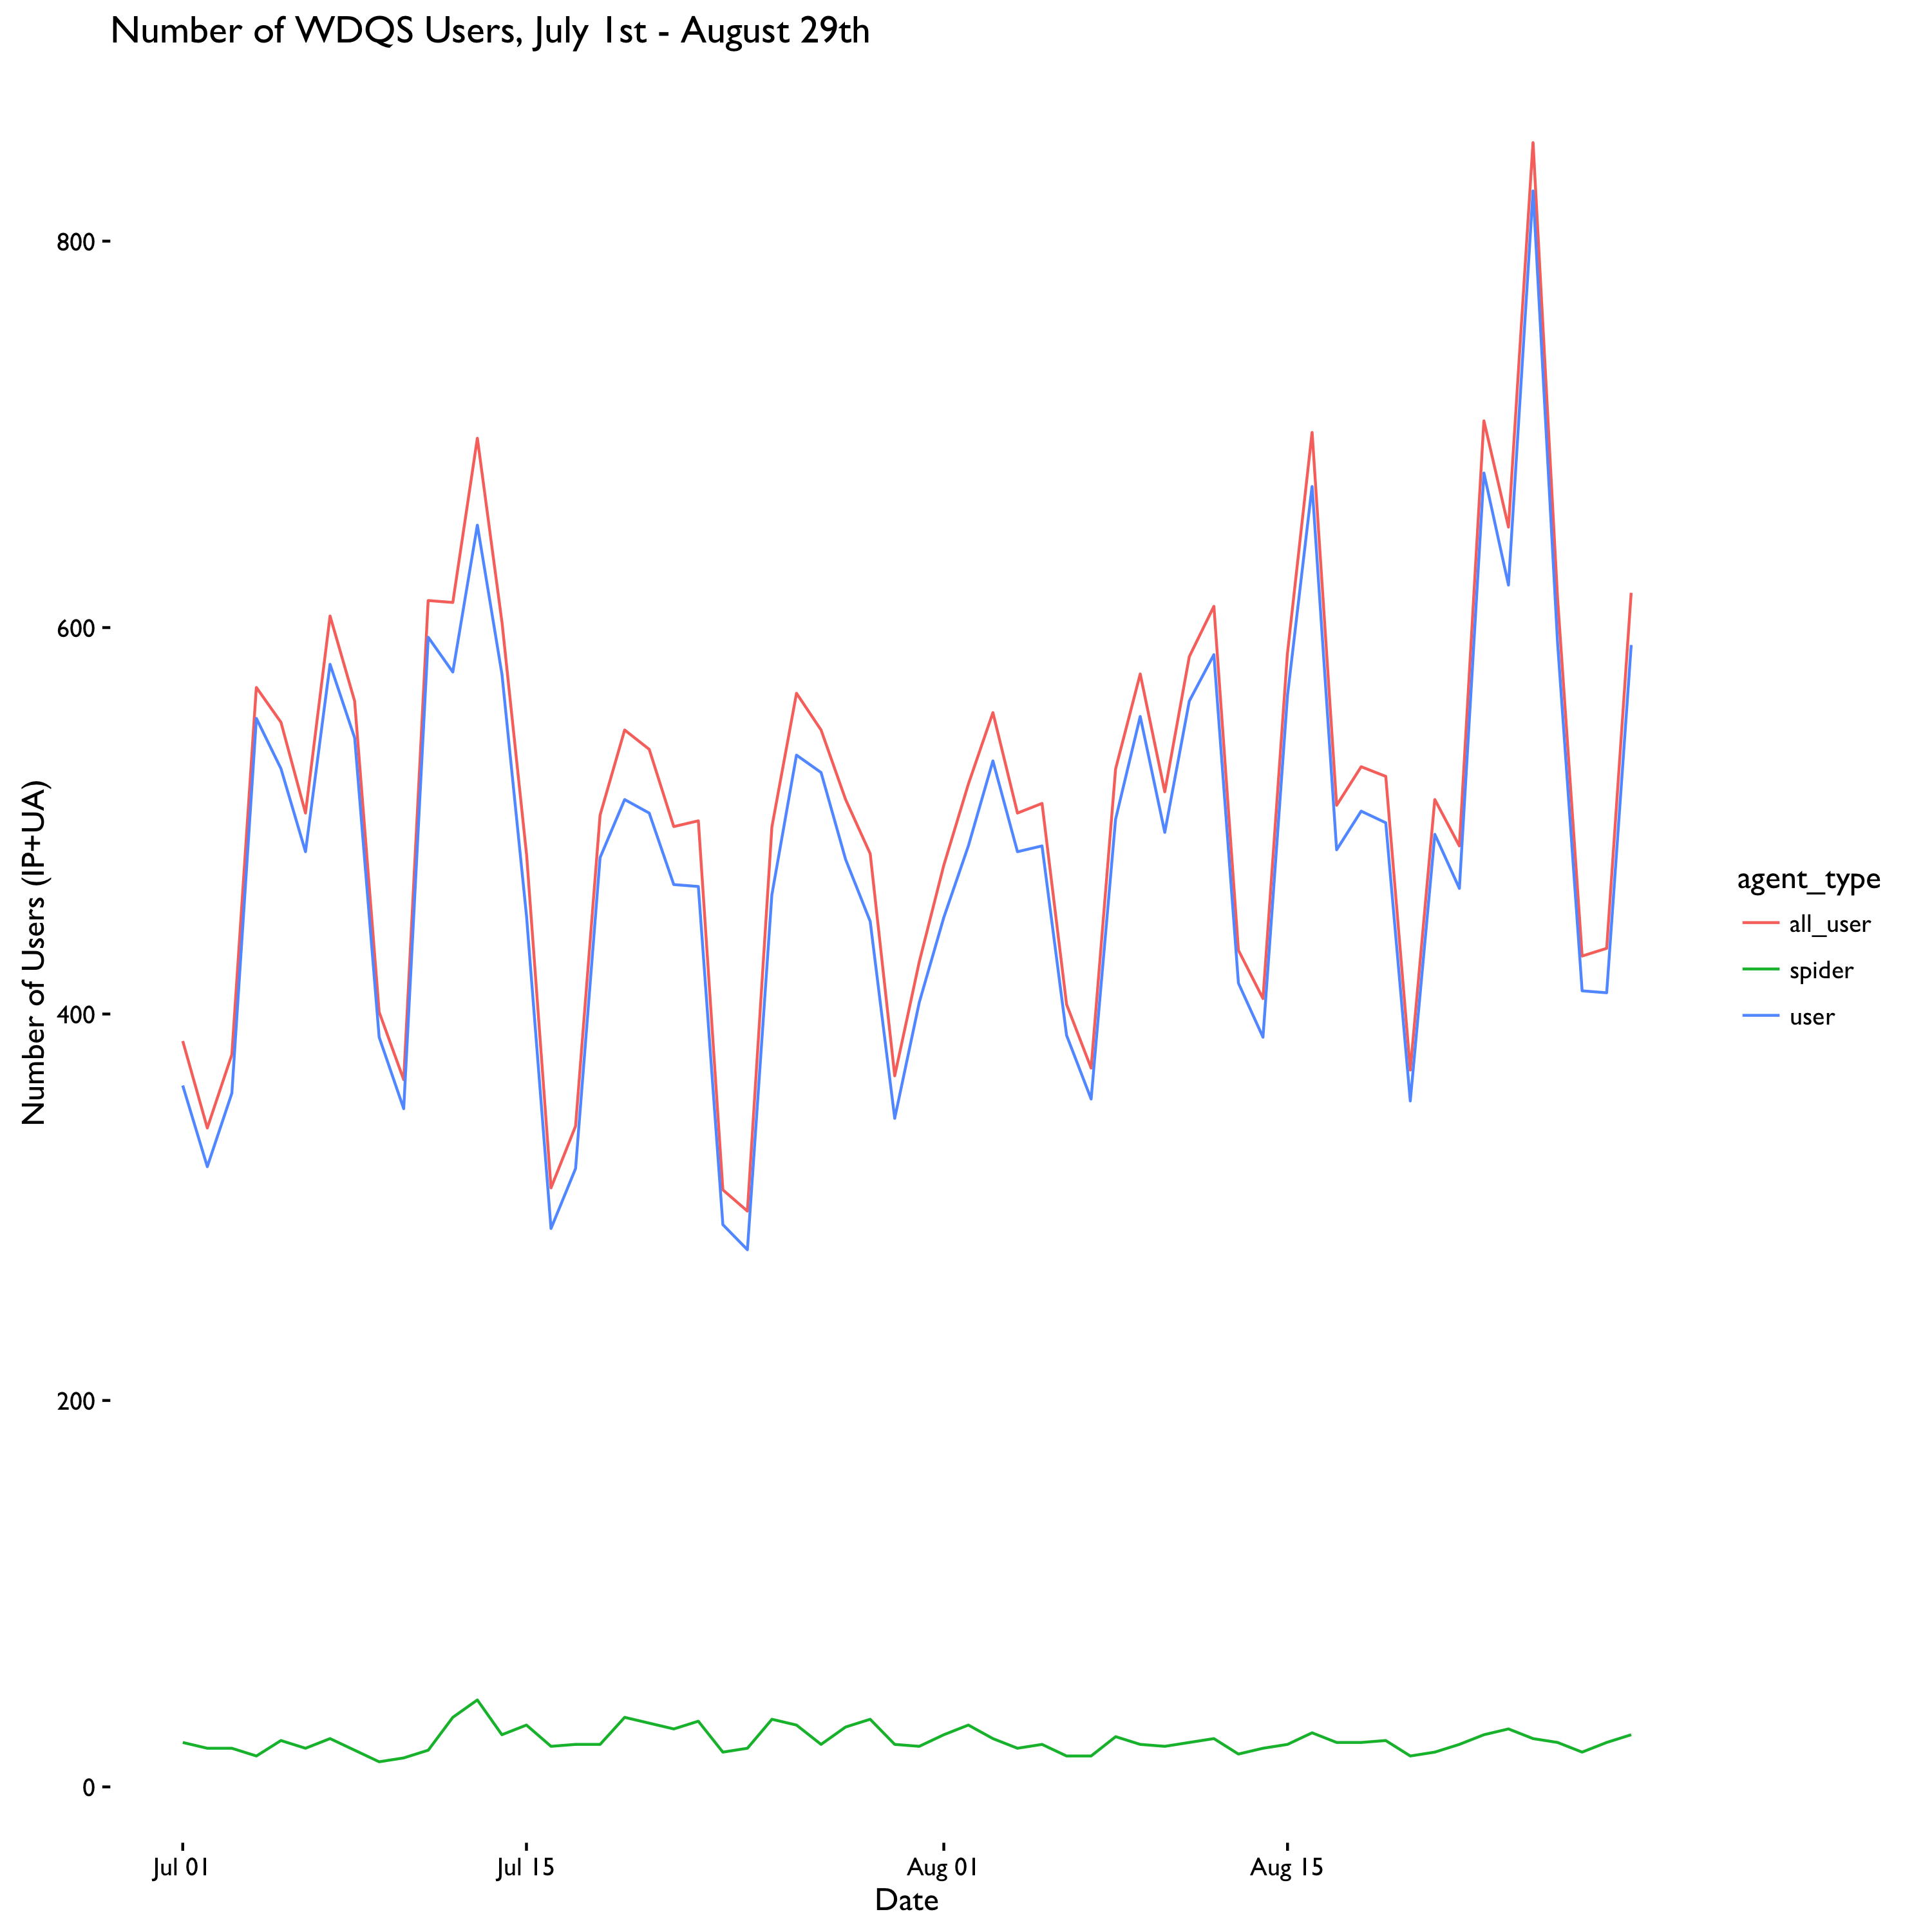
\includegraphics[width=9cm,height=9cm,keepaspectratio]{figures/all_user_ts.png}
\caption{There seems to be a weekly cycle in the number of users.}
\end{figure}

\begin{figure}[H]
\centering
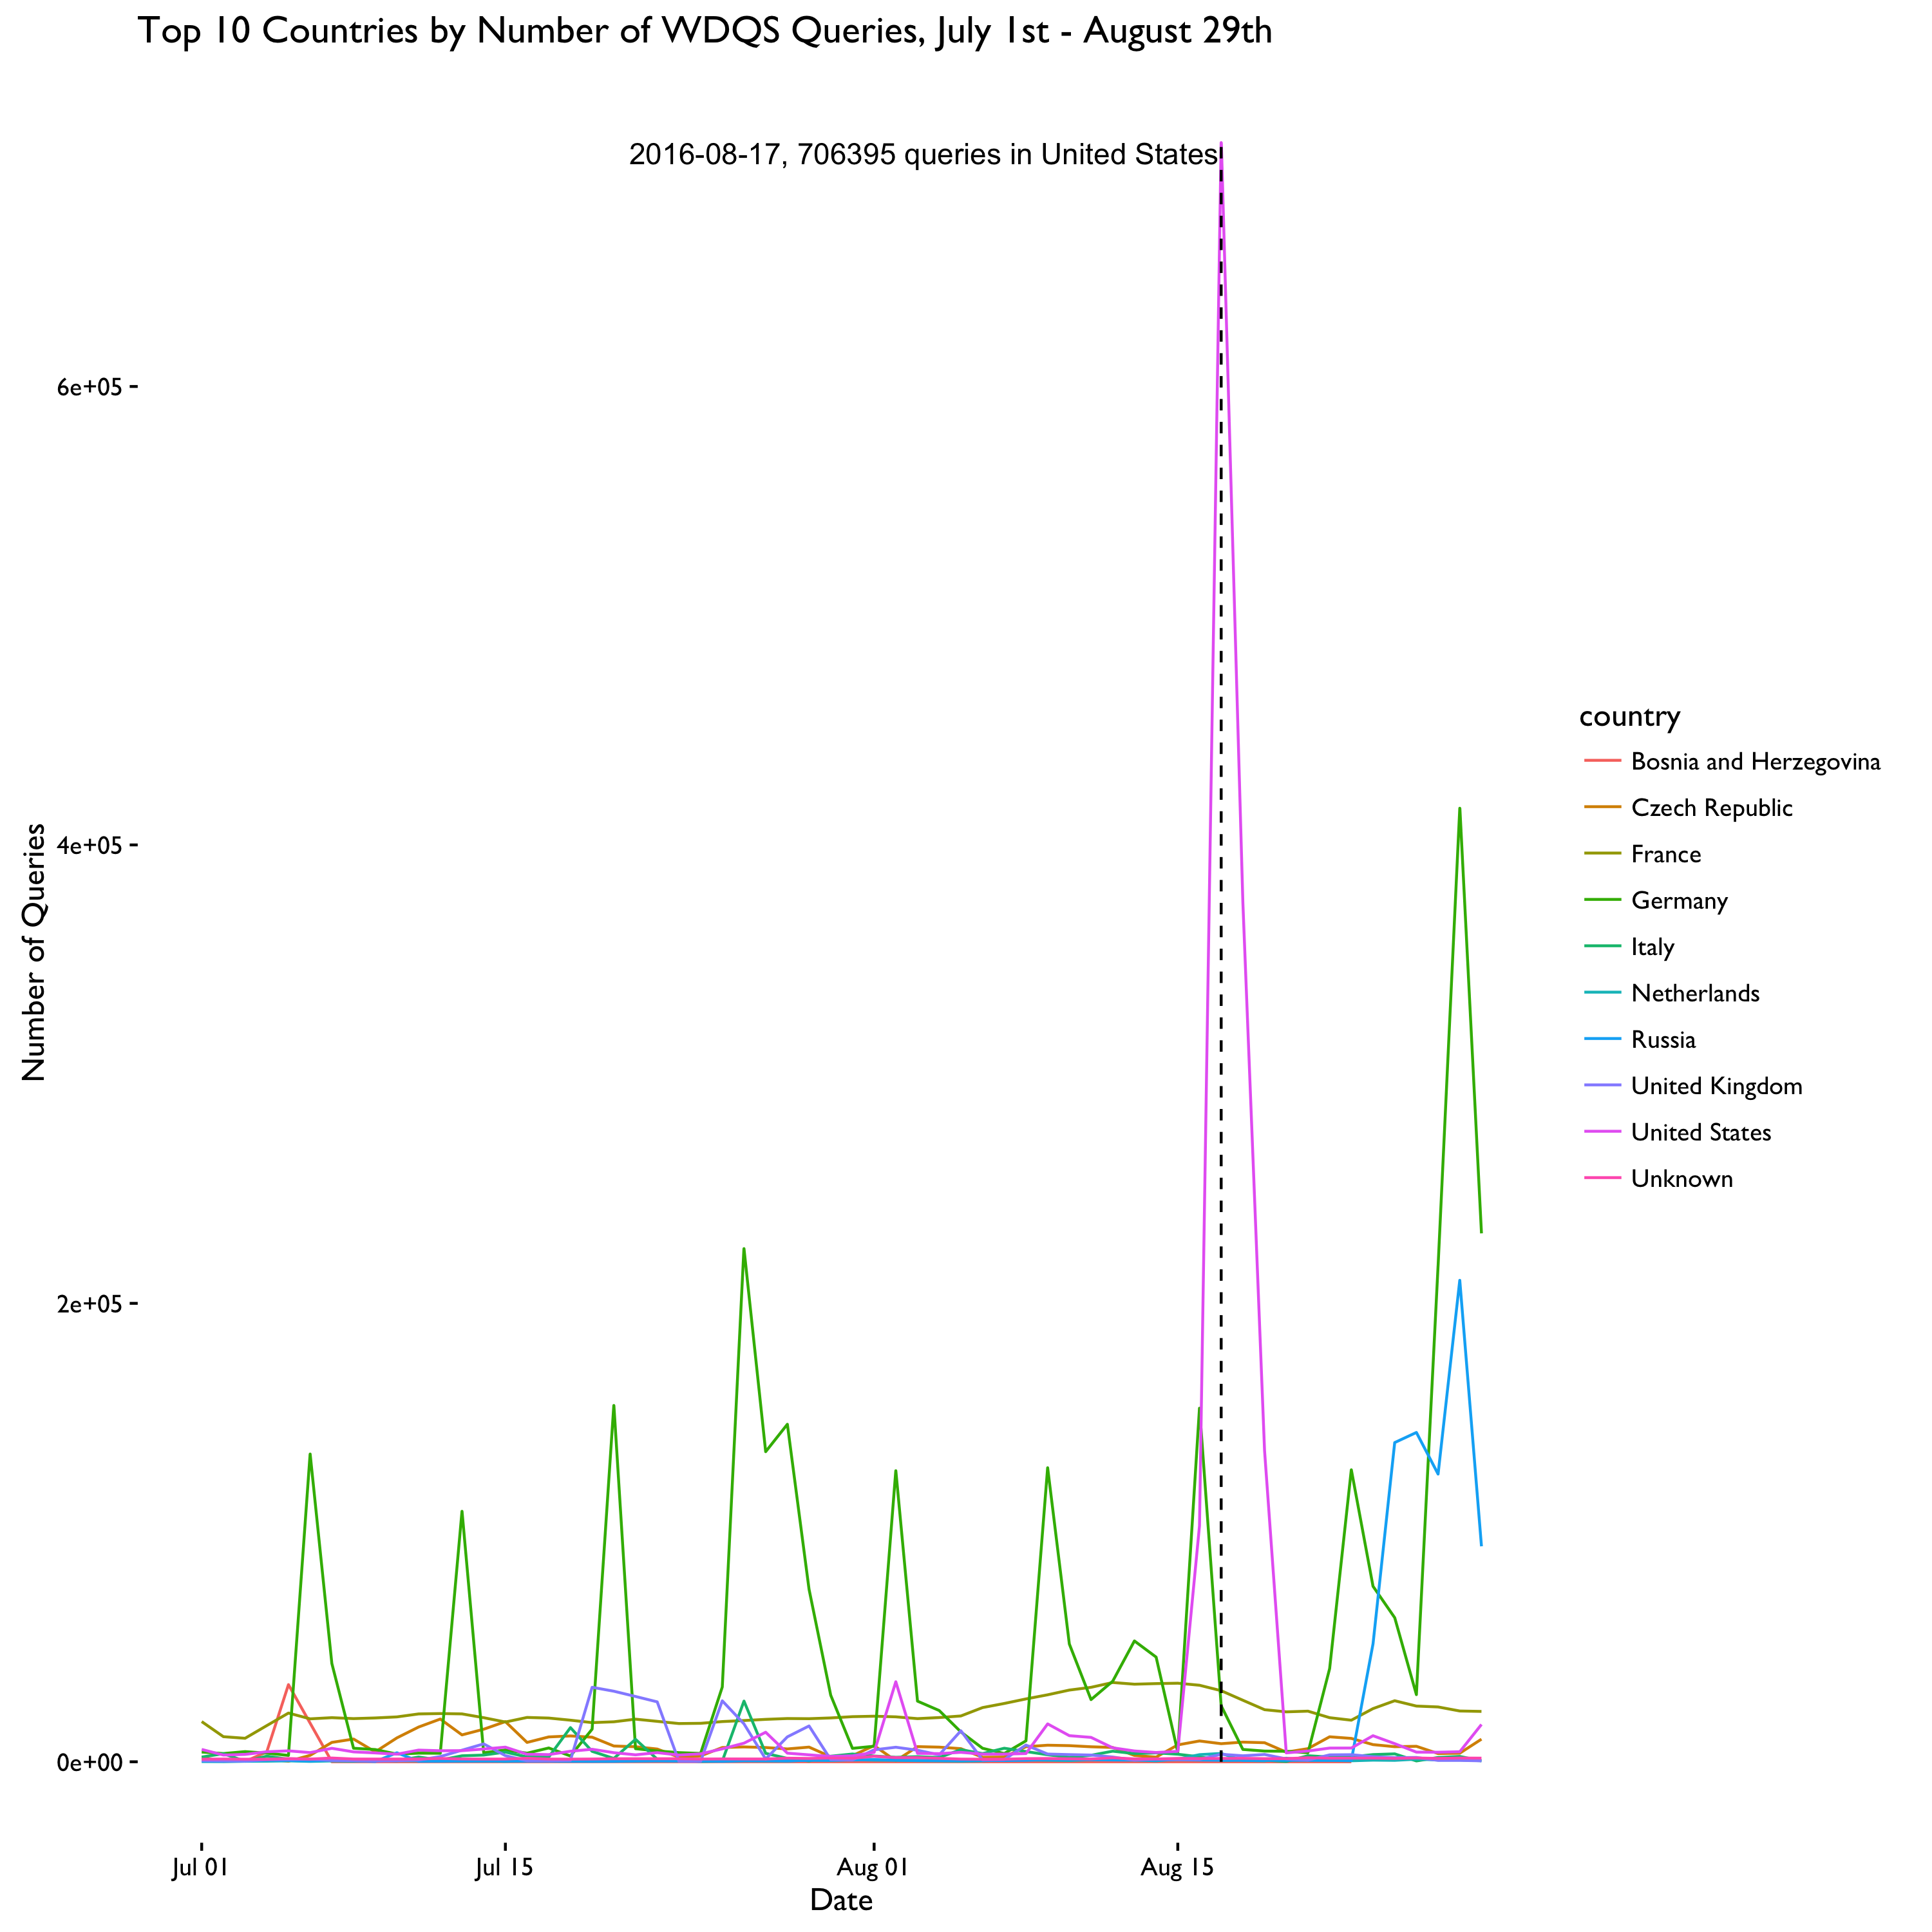
\includegraphics{figures/query_country_ts.png}
\caption{Further breakdown by country. The spike was contributed by the
US. Germany seems to dominate the weekly cycle. Bosnia and Herzegovina
saw a huge decrease in these two months.}
\end{figure}

\begin{figure}[H]
\centering
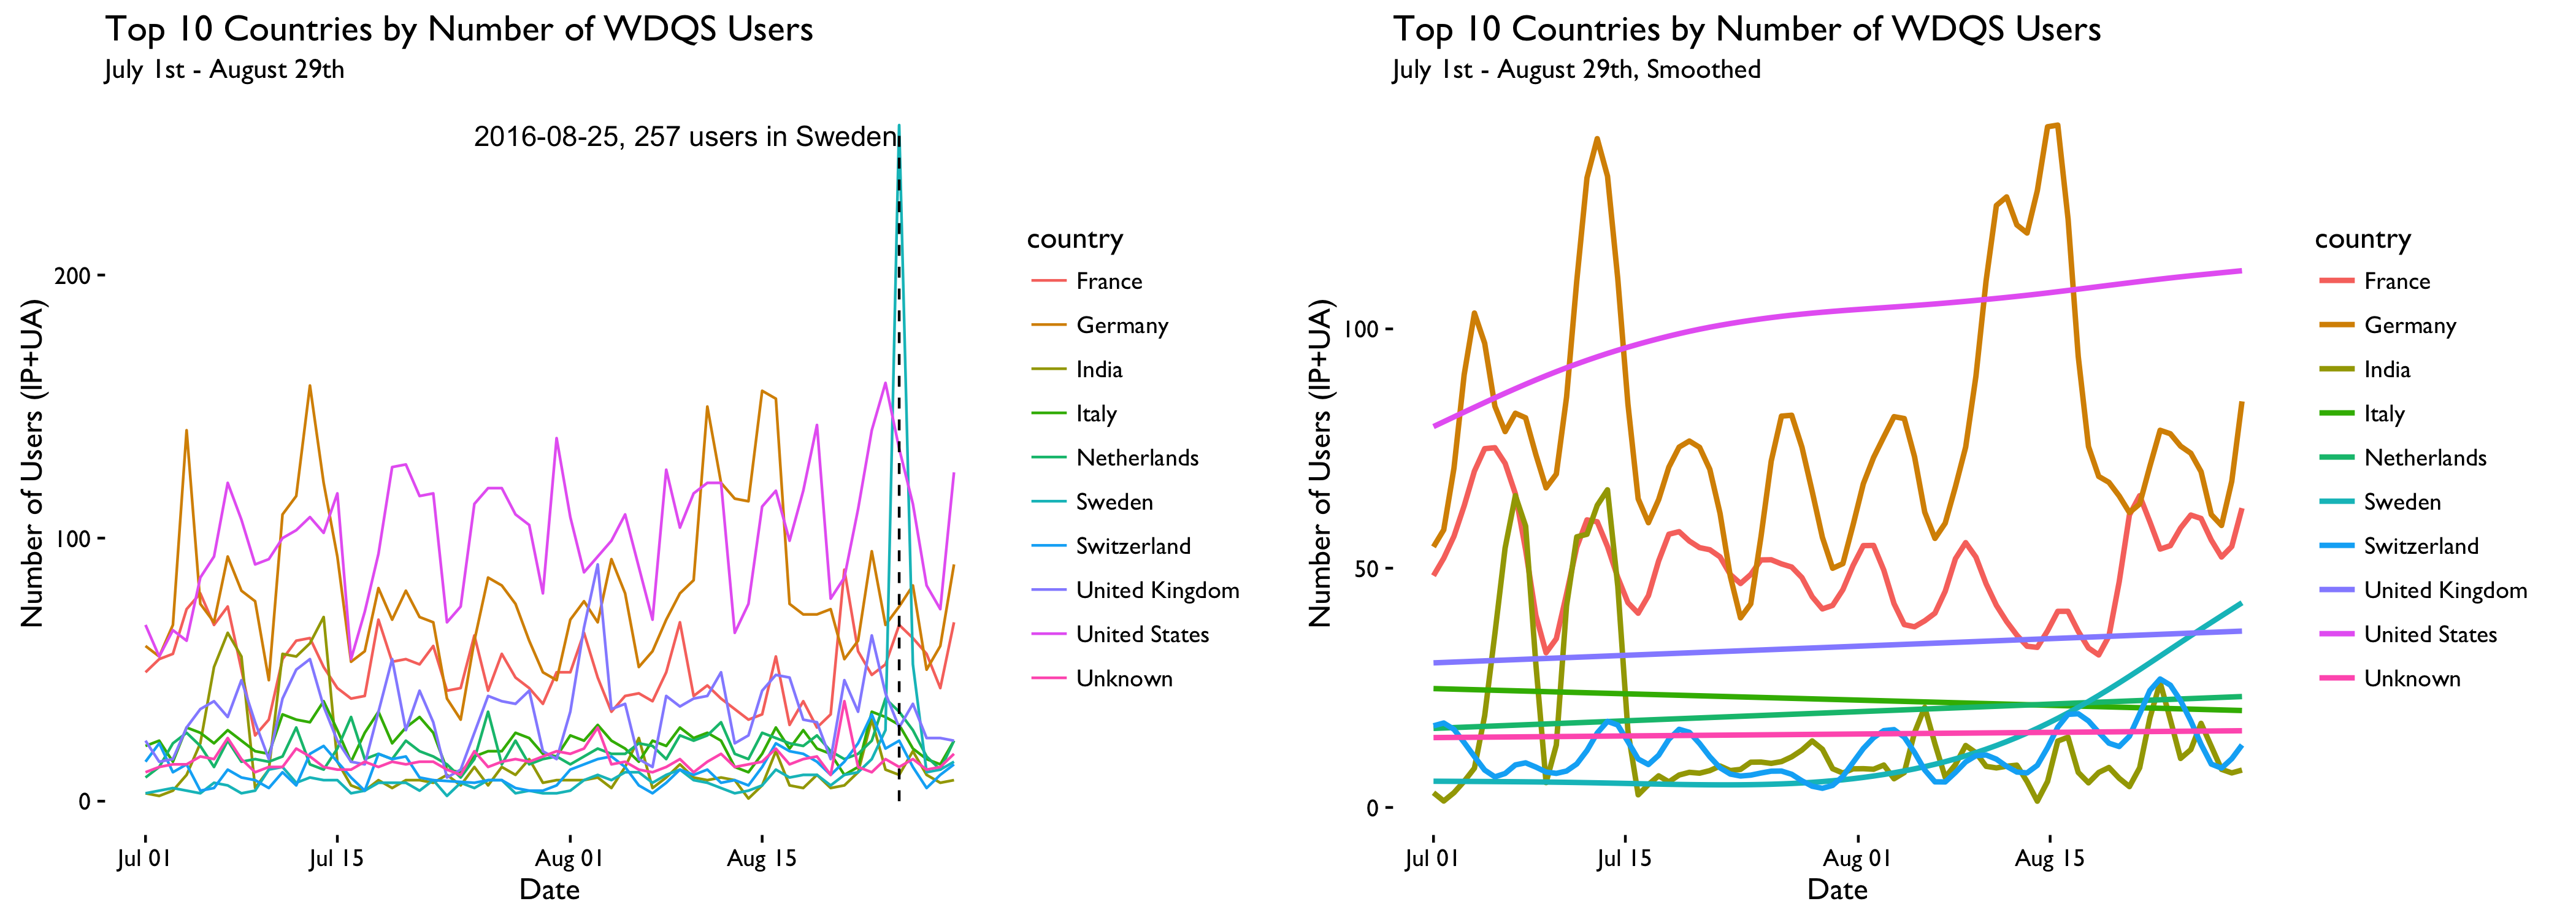
\includegraphics{figures/user_country_ts.png}
\caption{Top 10 Countries by Number of WDQS Users, July 1st - August
29th, 2016.}
\end{figure}

Next, we excluded the automata queries in US from August 16 to 19
(Figure \ref{eclus}), then implemented BFAST method on the query data.
BFAST (Breaks For Additive Season and Trend) integrates the
decomposition of time series into trend, season, and remainder
components with methods for detecting and characterizing change within
time series. First, it decomposes the series into trend and seasonal
components with the STL method, then it uses OLS-MOSUM test on each
components to see if there is any significant break point. Next, BFAST
fits the two components and the detected break points with linear
regression. BFAST iteratively estimates the time and number of changes,
and characterizes change by its magnitude and direction, until the
number and position of the breakpoints are unchanged.

\begin{figure}[H]
\centering
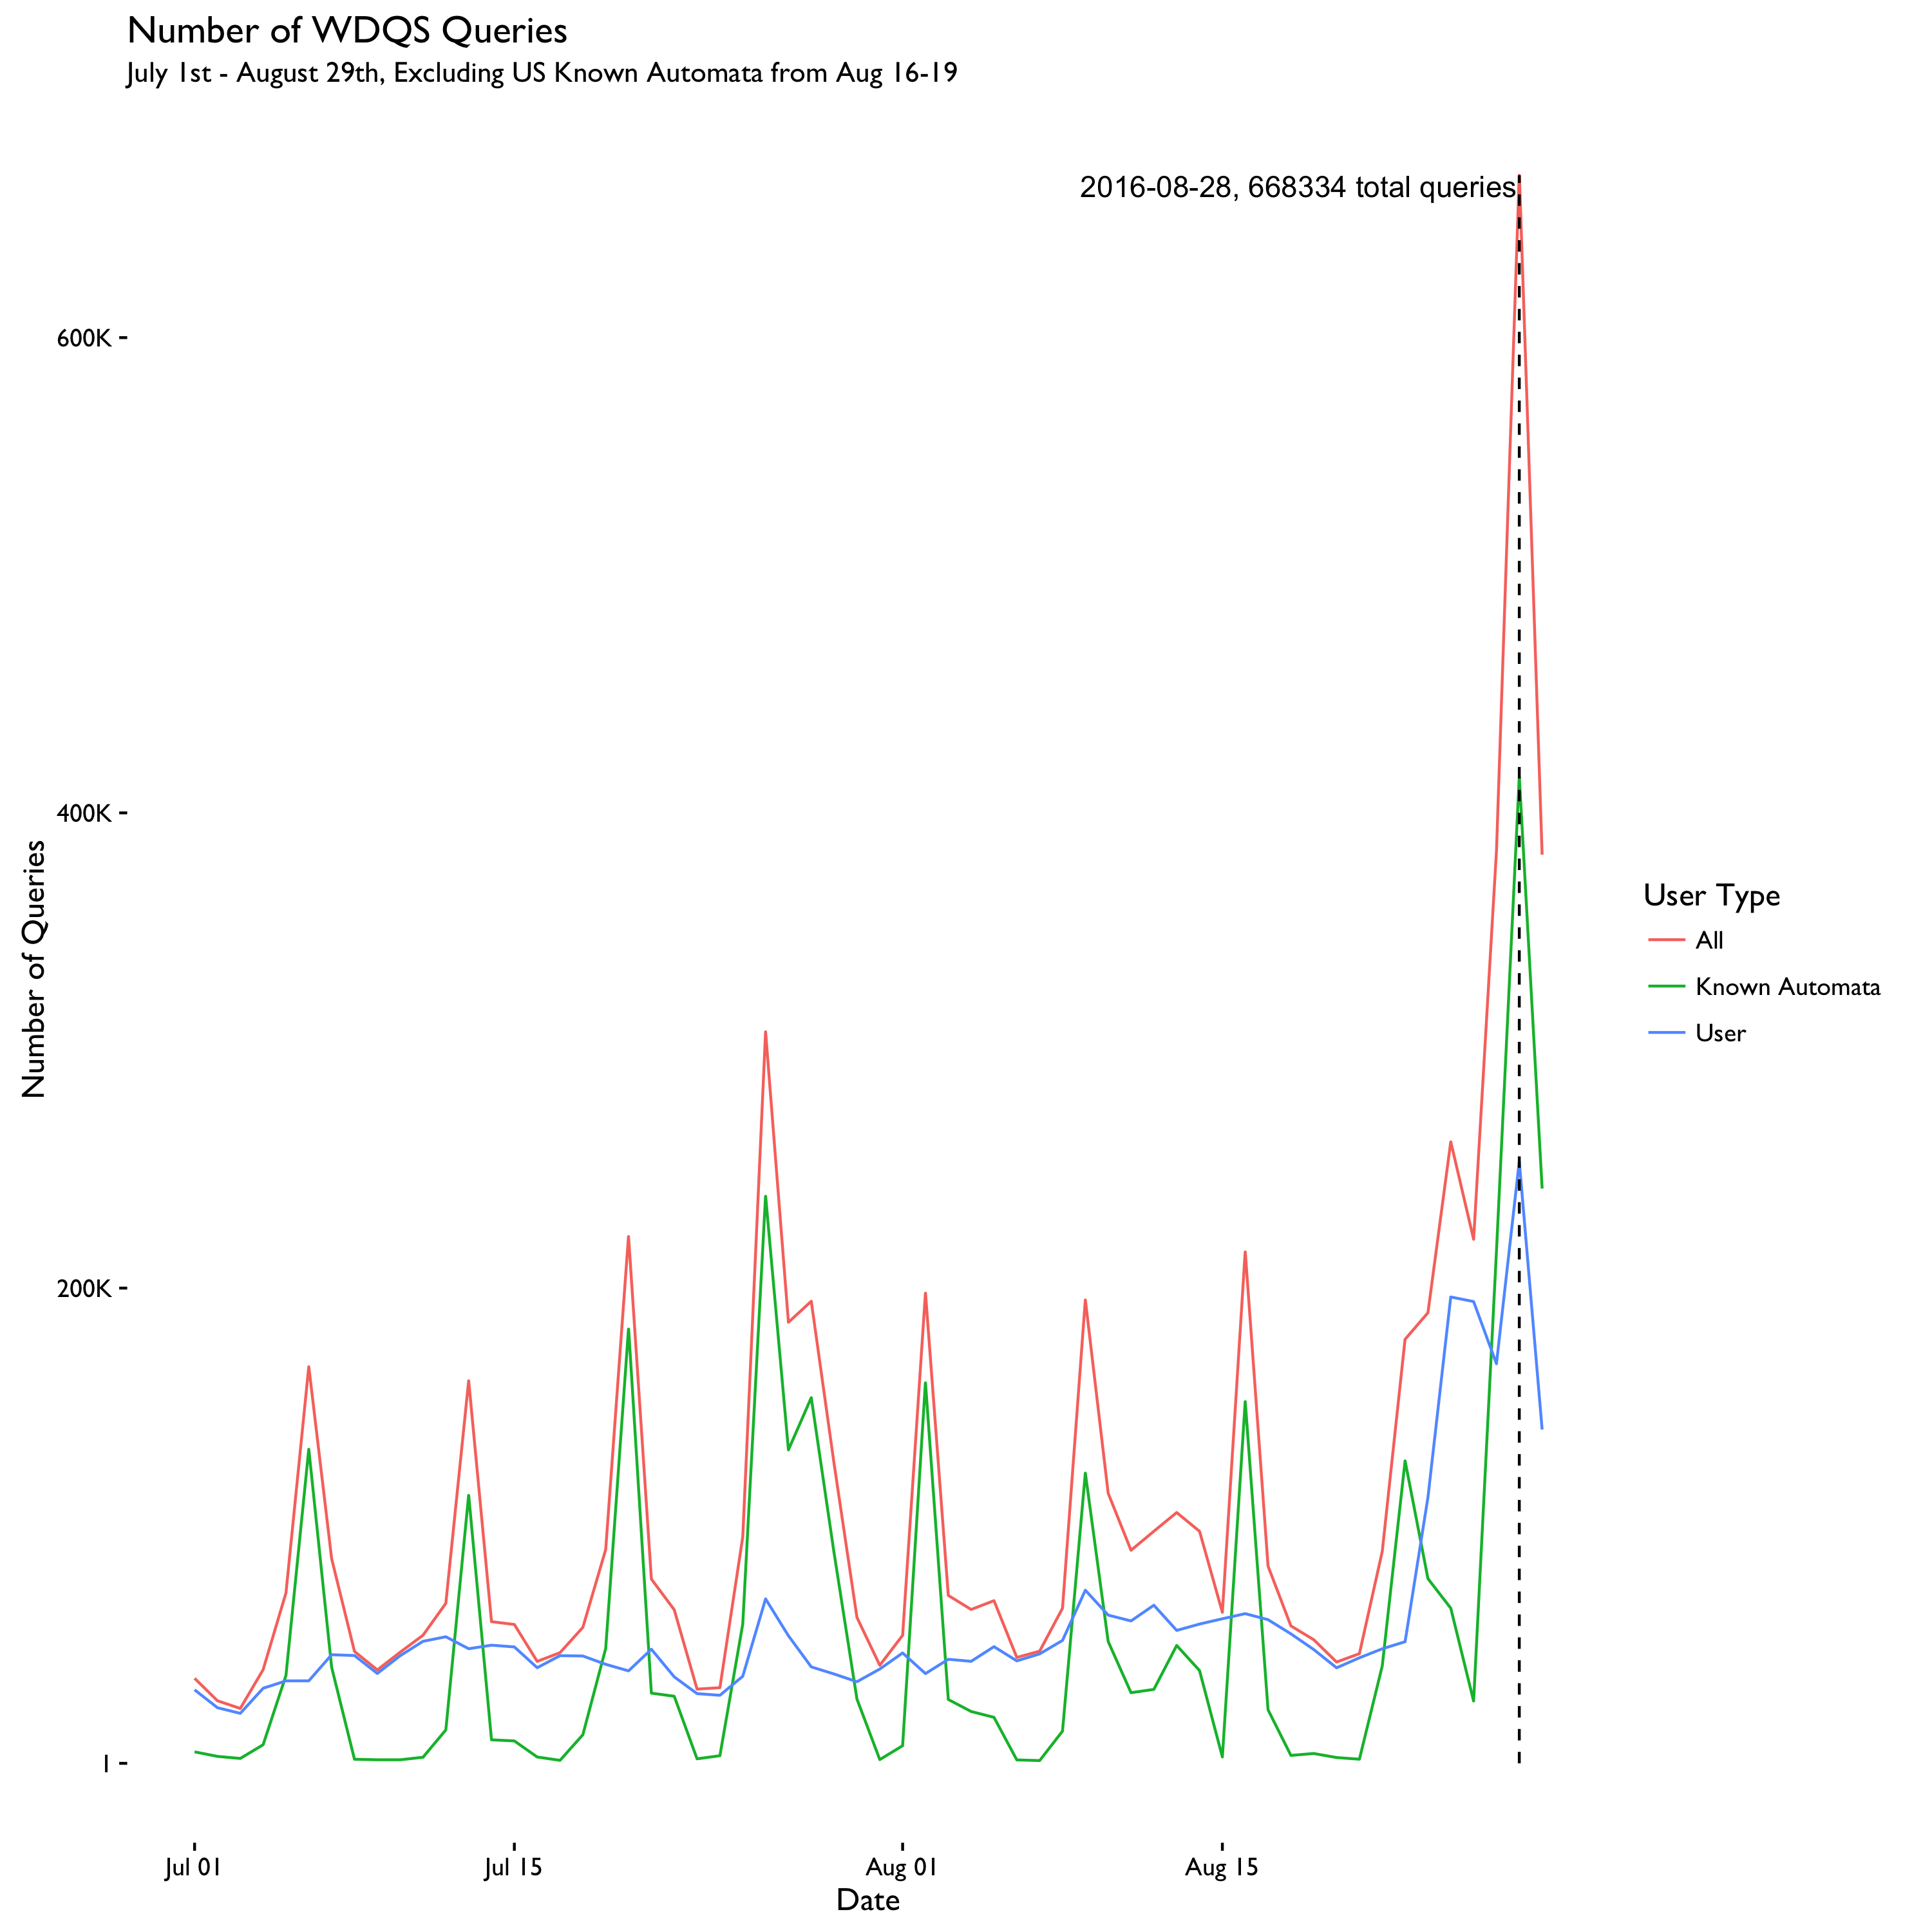
\includegraphics[width=9cm,height=9cm,keepaspectratio]{figures/all_query_ecl_us_spider0816_ts.png}
\caption{After excluding the automata queries from US Aug 16-19, the
weekly cycle seems to hold for those days. Further investigation is
needed to find out whether this spike is contributed by a particular
automata.\label{eclus}}
\end{figure}

\begin{figure}[H]
\centering
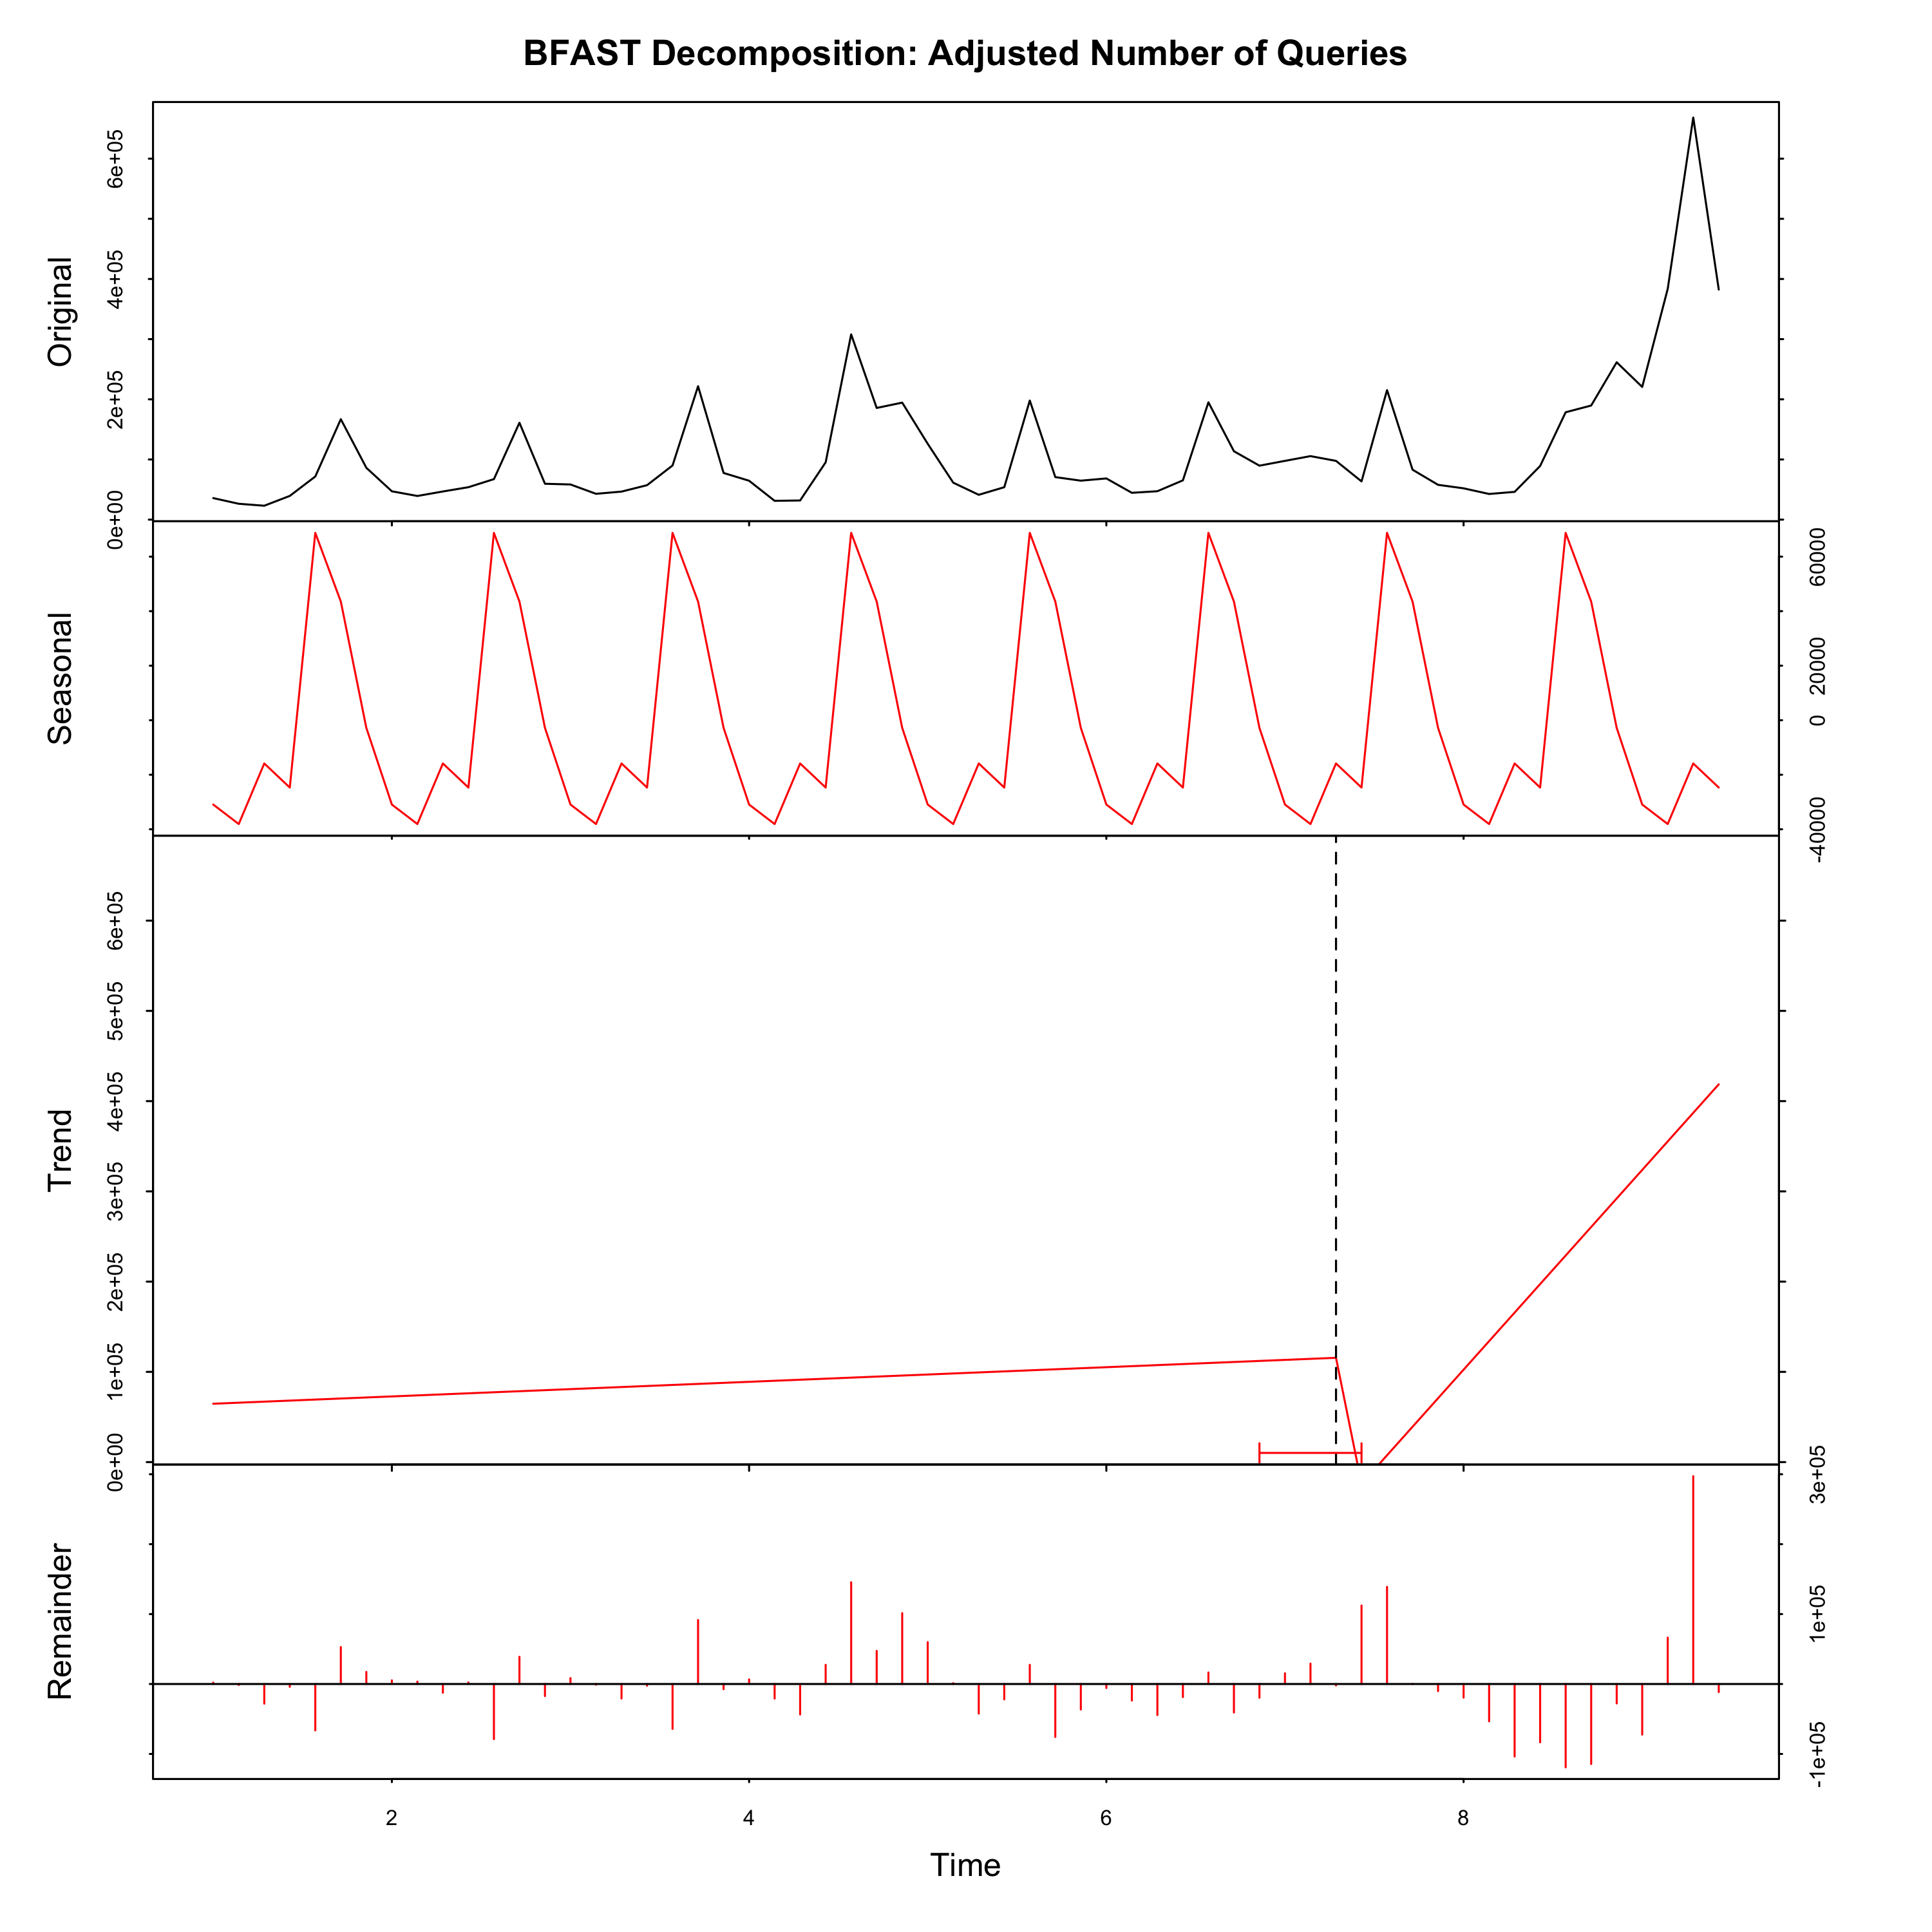
\includegraphics[width=9cm,height=9cm,keepaspectratio]{figures/adjust_query_decompose.png}
\caption{Adjusted number of queries decomposition. BFAST method detect a
change point on Aug 14 in the trend component. At the change point, the
decrease may be a result of our adjustment (excluding US automata), and
more observations are needed to confirm the increase afterwards.}
\end{figure}

\begin{figure}[H]
\centering
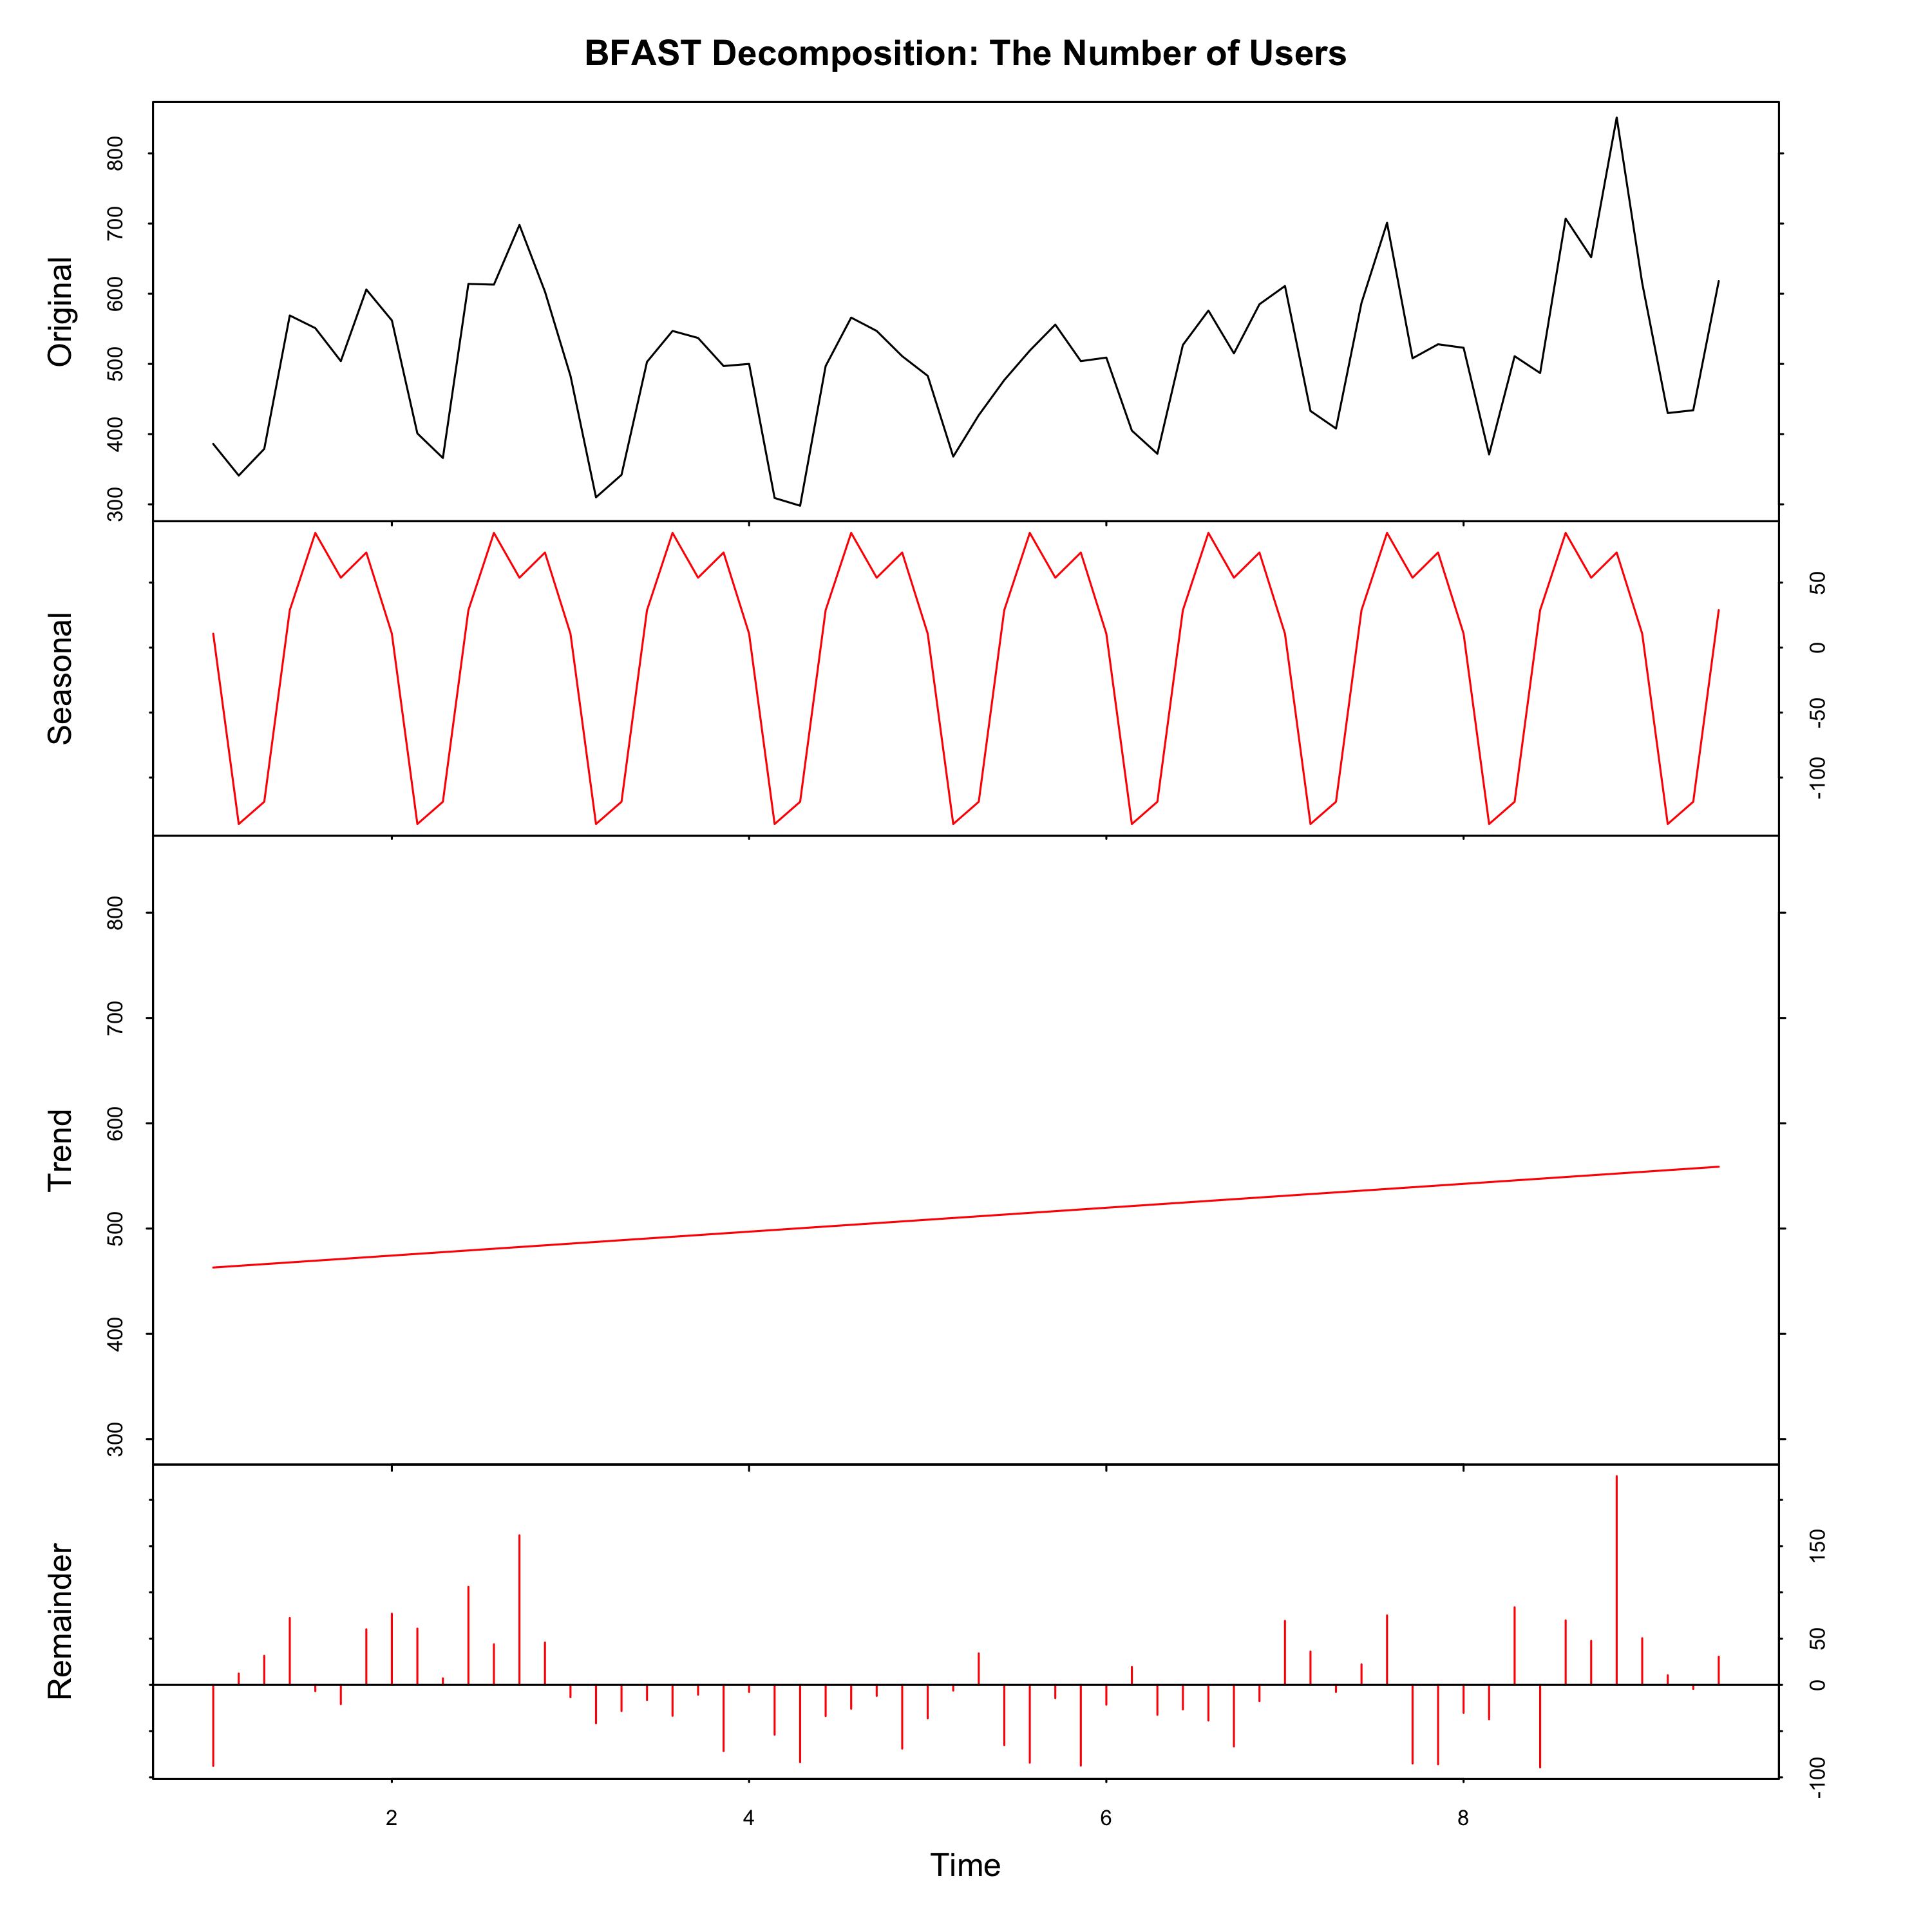
\includegraphics[width=9cm,height=9cm,keepaspectratio]{figures/user_decompose.png}
\caption{Number of users decomposition. There is no change point
detected. We also see a slightly increasing trend.}
\end{figure}

\begin{figure}[H]
\centering
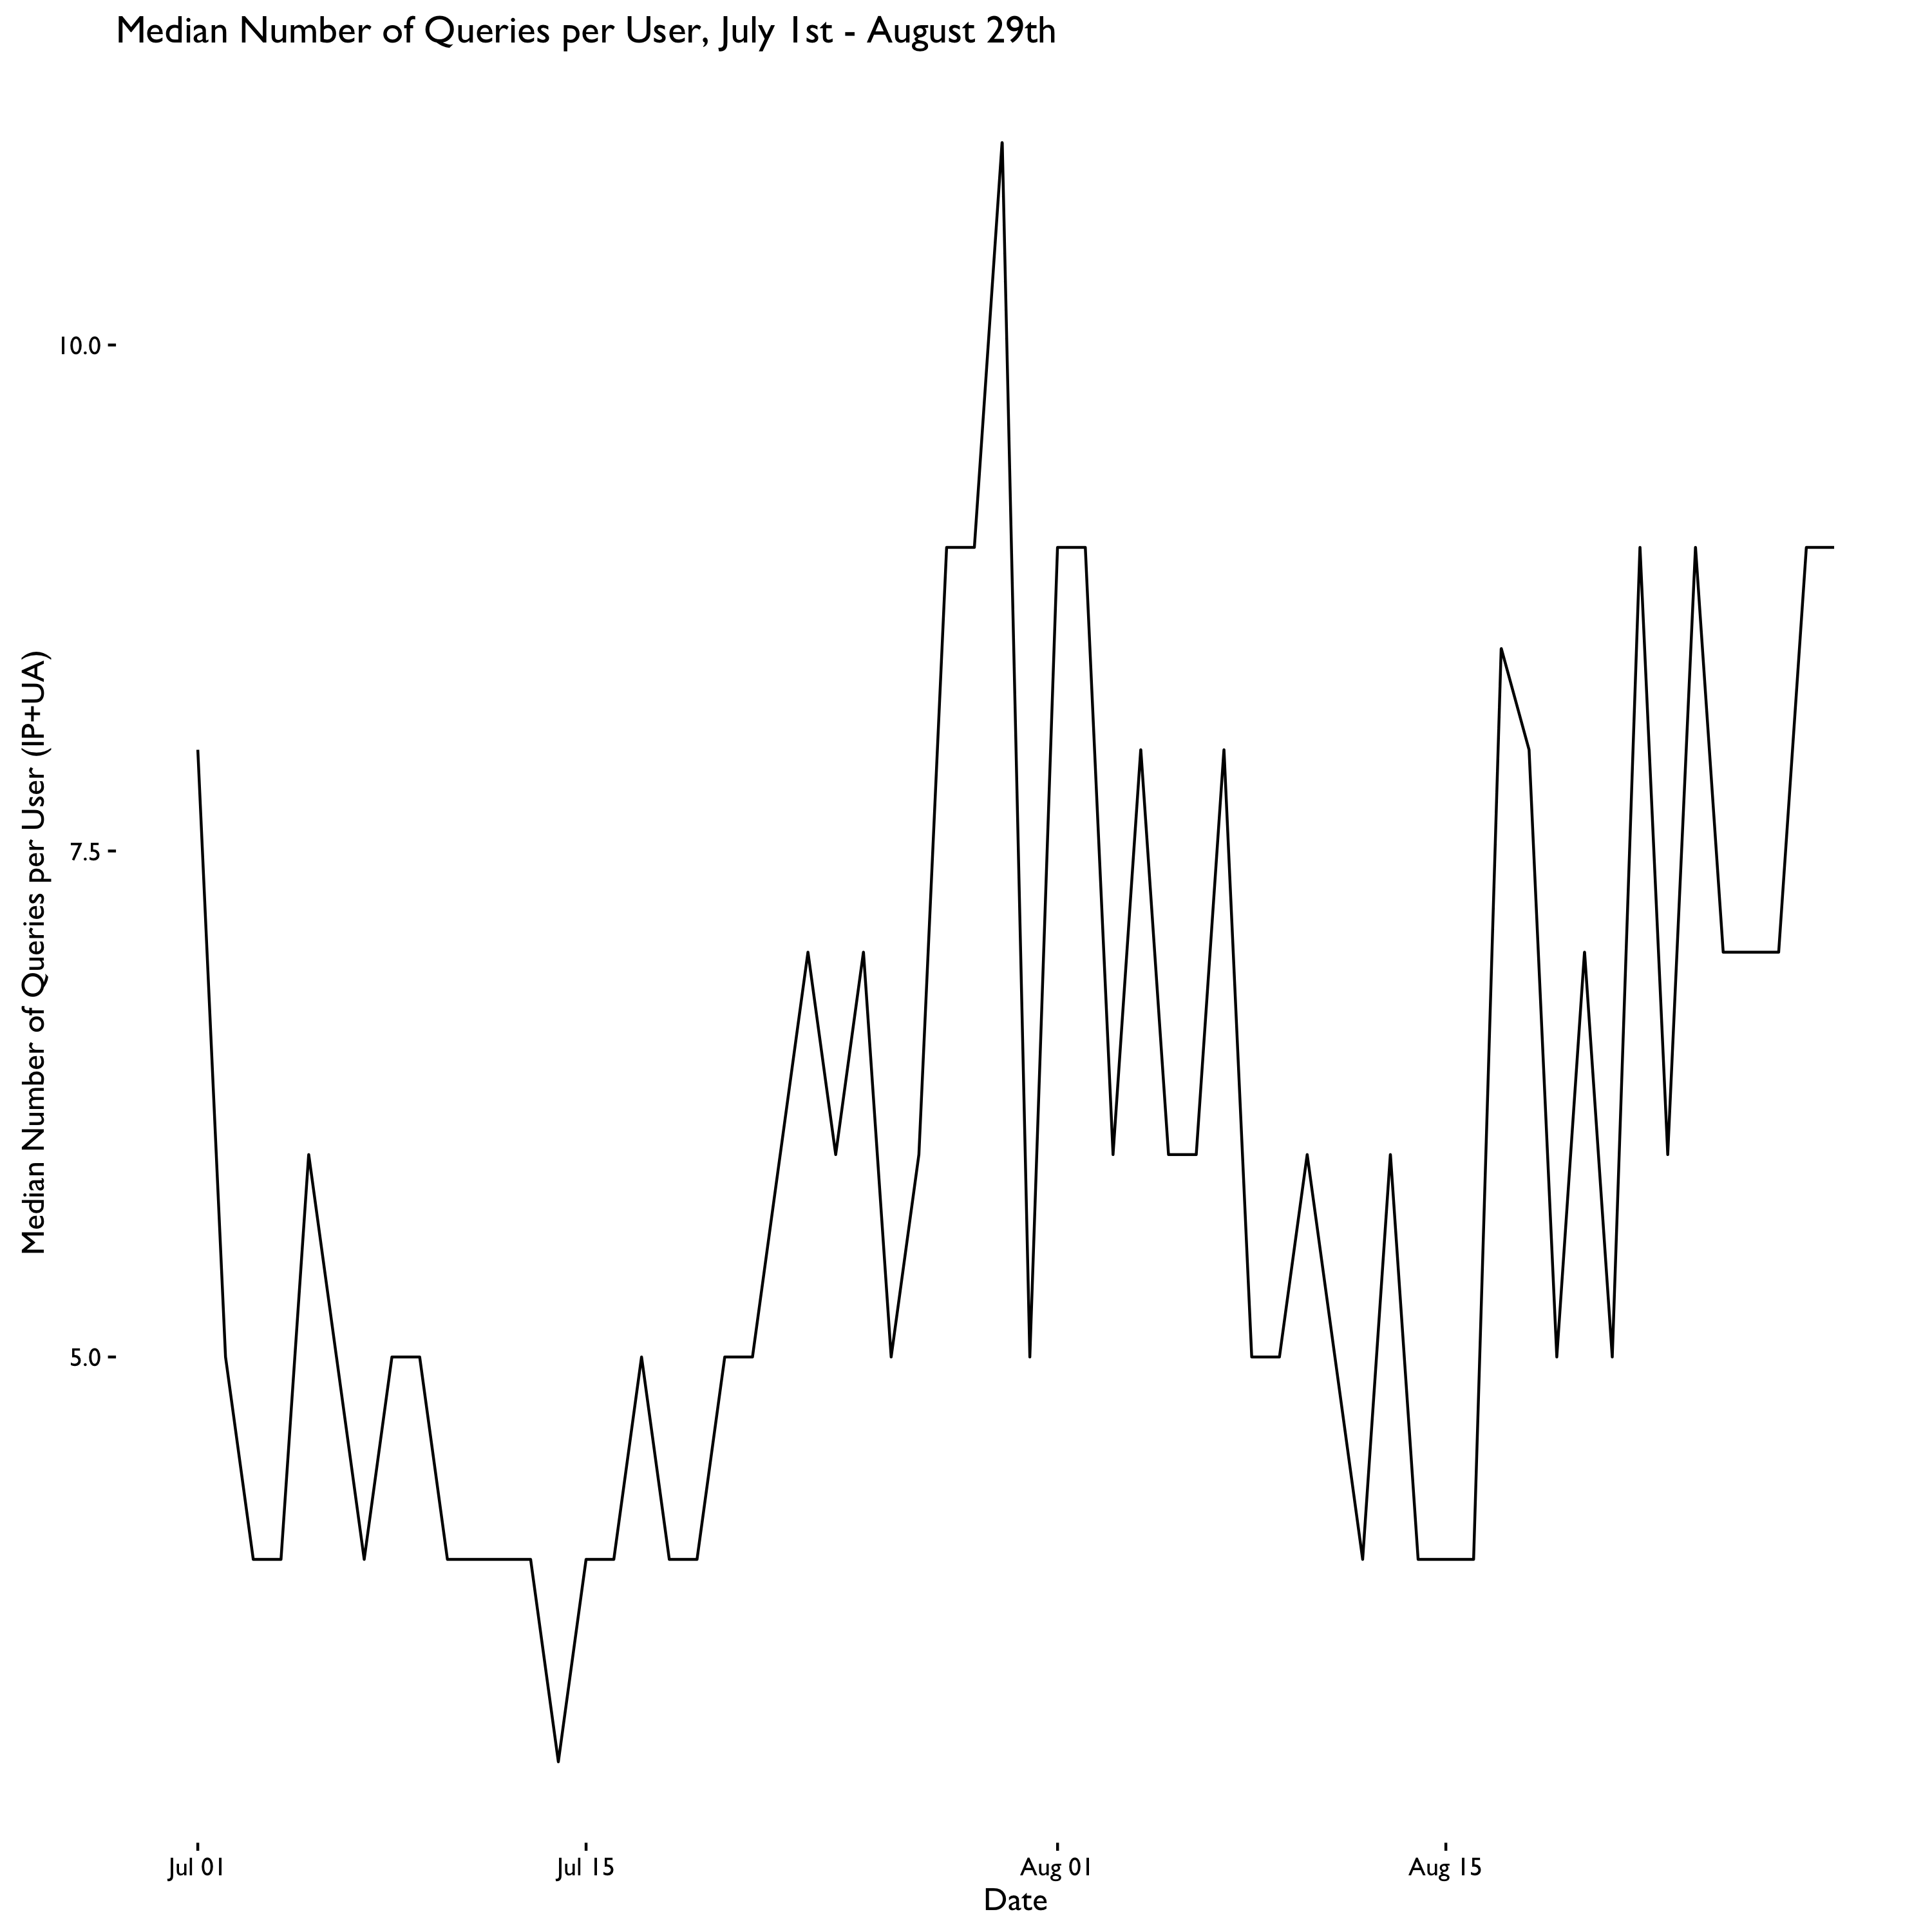
\includegraphics[width=9cm,height=9cm,keepaspectratio]{figures/md_query_per_user_ts.png}
\caption{Median Number of Queries per User.}
\end{figure}

\begin{figure}[H]
\centering
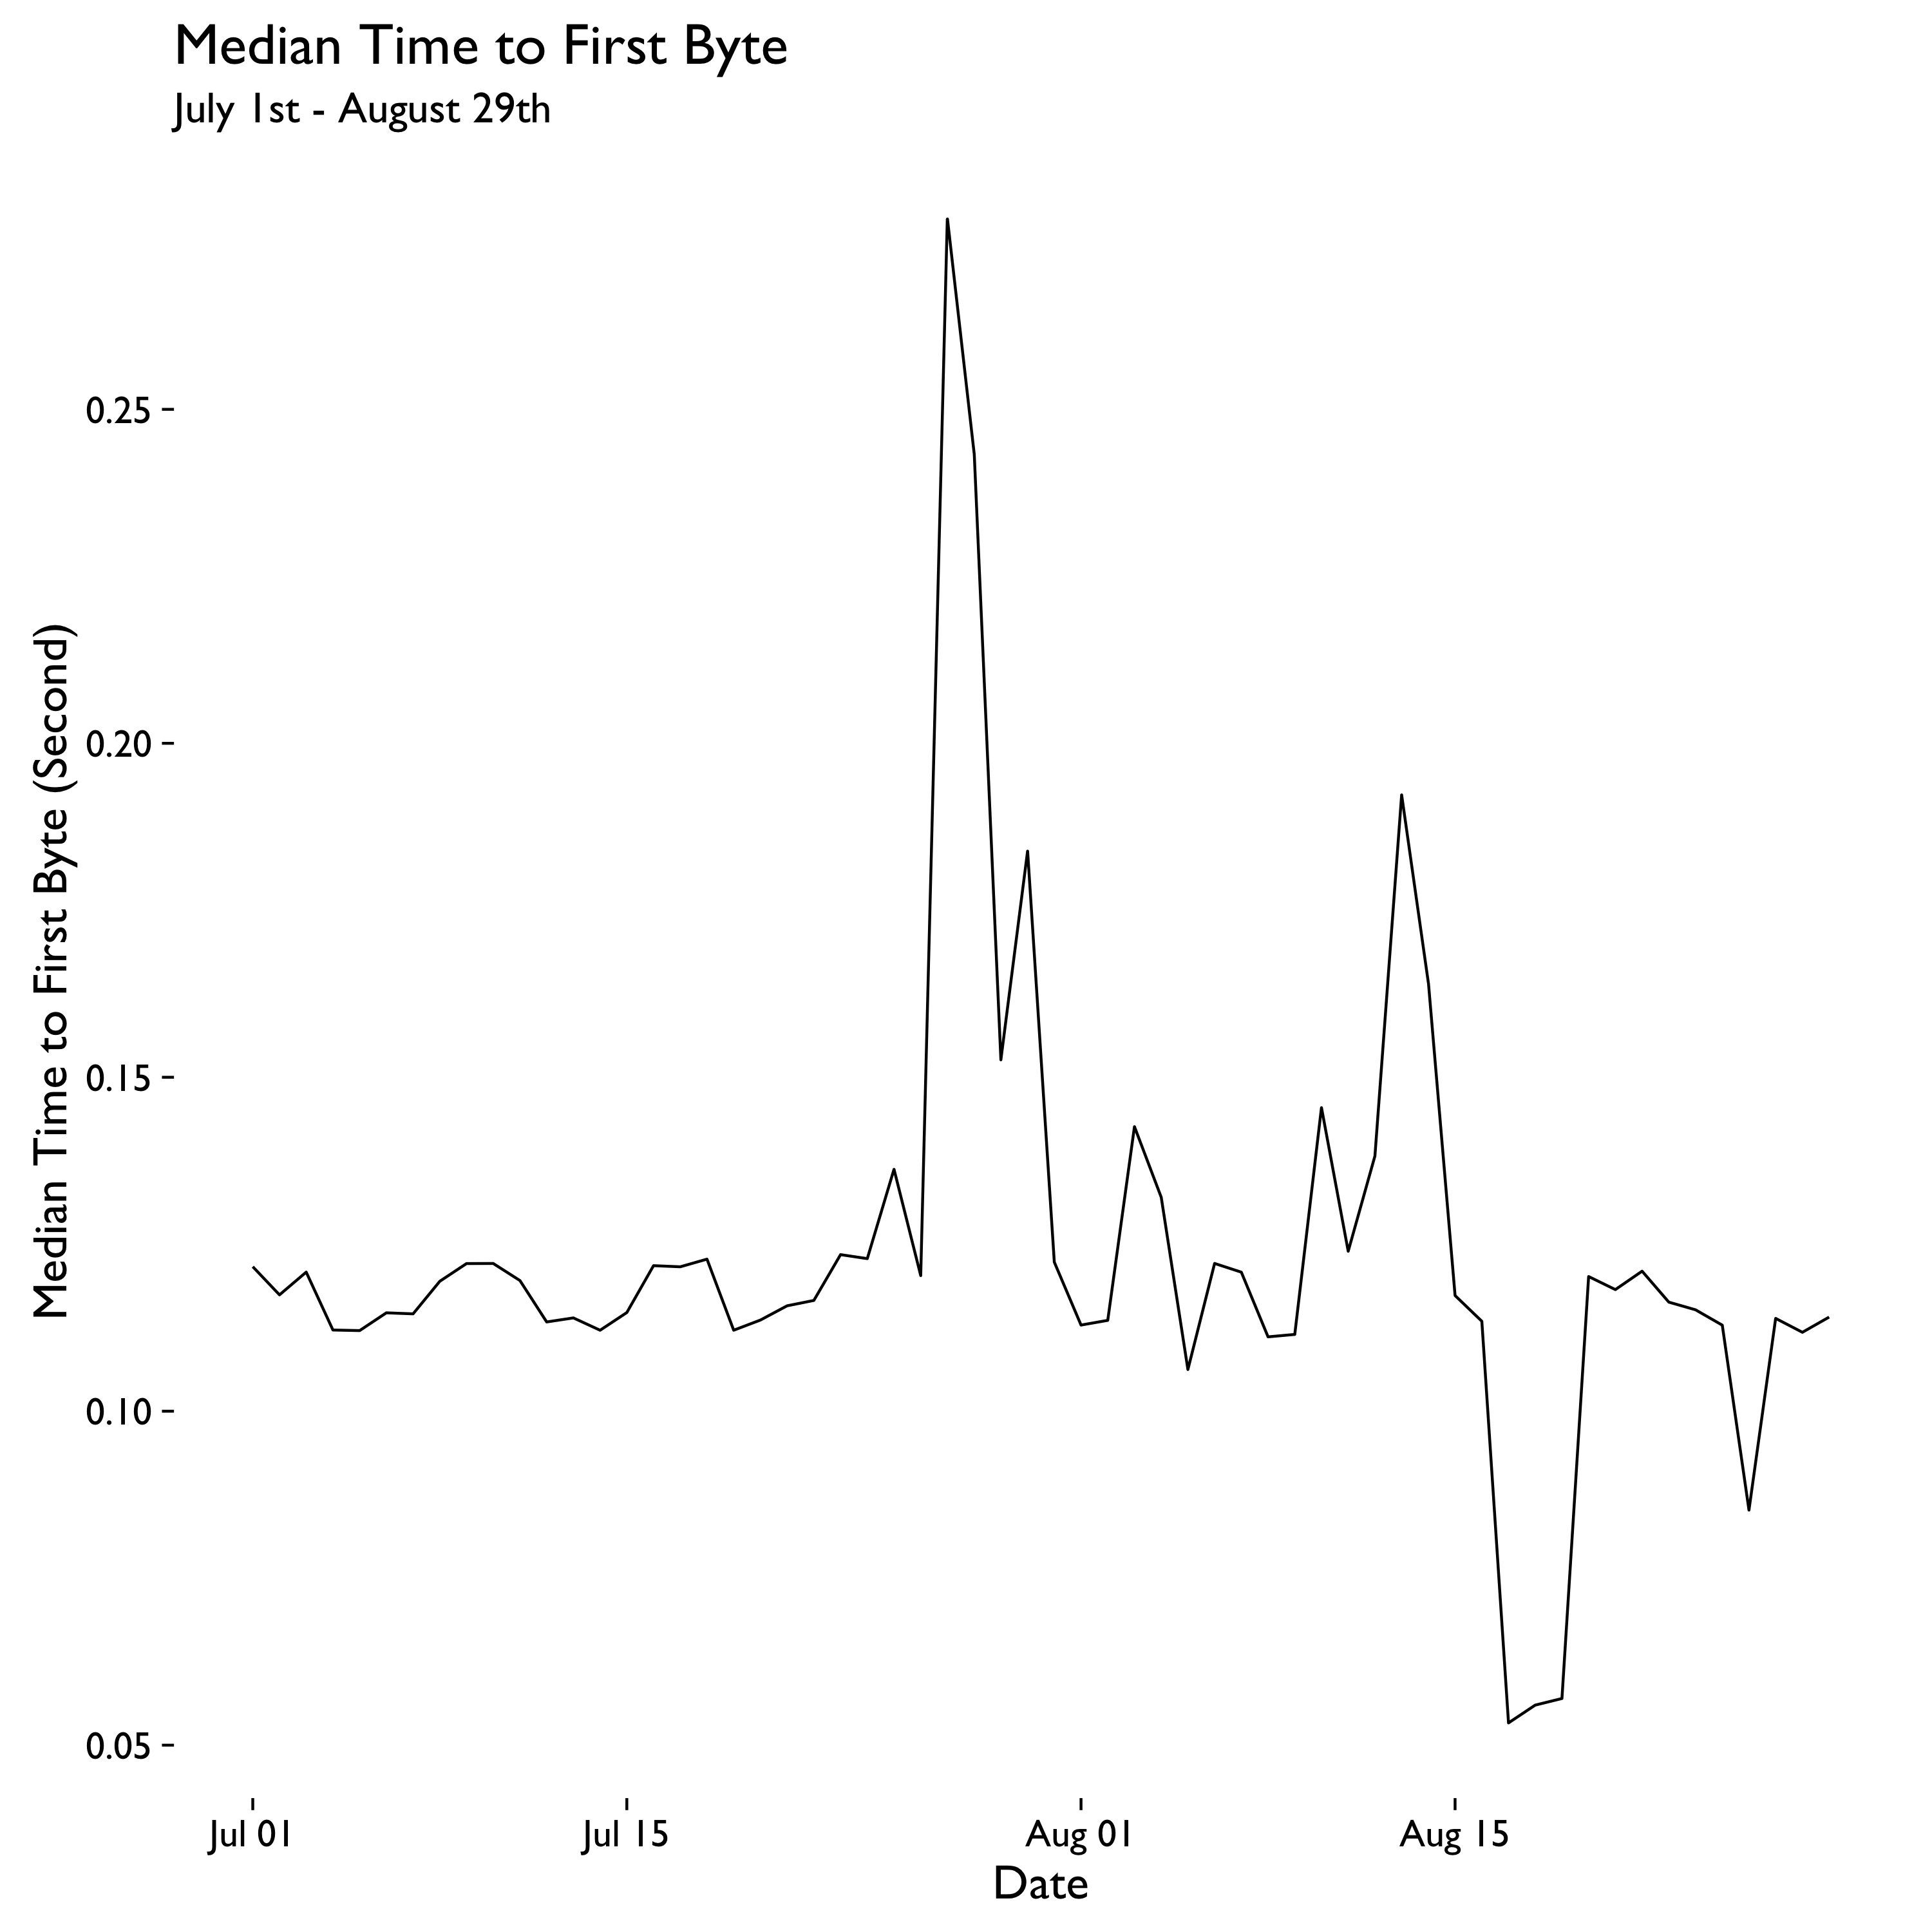
\includegraphics[width=9cm,height=9cm,keepaspectratio]{figures/median_time_firstbyte_ts.png}
\caption{Time to first byte is a measurement used as an indication of
the responsiveness of our servers. We saw a sharp decrease around August
17, which may be the result of the large number of automata queries. We
also saw two spikes around July 25 and August 13, of which further
investigation is needed.}
\end{figure}

\newpage

\subsection{Conclusion/Discussion}\label{conclusiondiscussion}

In summary, we found that:

\begin{itemize}
\tightlist
\item
  Germany, United States and France have the largest number of users and
  queries.
\item
  Among regular users (not known automata), Mac OS X and Chrome are most
  popular, while Ubuntu and Firefox users submit the most queries.
\item
  Most queries have no referer, followed by those referred from search
  engine.
\item
  There are weekly cycles in the number of queries and users. And we
  also saw an increasing trend in the number of users.
\end{itemize}

For the next step, more thorough analysis and investigation are needed
in order to solve the following questions:

\begin{itemize}
\tightlist
\item
  It looks like Ubuntu users have more queries-per-user than other
  operating systems on average. Is it the result of several outliers?
\item
  We saw a large number of automata queries from US on Aug 16-19. Are
  they from one or several particular automata?
\item
  What is the reason for the decrease number of queries of Bosnia and
  Herzegovina?
\item
  Is there a significant increasing trend in the number of queries after
  August 19? Is the increasing trend in the number of users
  statistically significant?
\item
  If we exclude known automata queries from Germany, could we still see
  the weekly cycle?
\item
  What could possibly be the reason for the spikes and sharp decrease in
  the time to first byte pattern?
\end{itemize}

\end{document}
